% !TeX root = MAT 2138 - Discrete Mathematics.tex

\title{\textbf{Discrete Mathematics}}

\date{}
\maketitle

\begingroup
\let\clearpage\relax
\tableofcontents
\endgroup

\clearpage

\renewcommand{\nomname}{List of Symbols}
\nomenclature[01]{$\forall$}{For all/any}
\nomenclature[02]{$\exists$}{For some / There exists}
\nomenclature[03]{$a \in S$}{$a$ belongs to / is an element of set $S$}
\nomenclature[04]{$\cup$, $\cap$}{Union and intersection (respectively) of sets}
\nomenclature[05]{$\varnothing$}{Empty set $\{\}$}
\nomenclature[06]{$\mathbb N$, $\mathbb Z$, $\mathbb Q$, $\mathbb R$, $\mathbb C$}{Sets of natural numbers, integers, rational numbers, real numbers, complex numbers (respectively)}
\nomenclature[07]{$\mathbb N_0$}{Set of non-negative integers $\{0, 1, 2, \ldots\}$}
%\nomenclature[08]{$\mathbb R_{>0}$}{Set of positive real numbers}
\nomenclature[08]{$A \subseteq B$}{$A$ is a subset of set $B$}
\nomenclature[09]{$\lvert S \rvert$}{Cardinality of set $S$}
\printnomenclature[10em]

\clearpage

\section{Elementary Set Theory}\label{sec:SetTheory}

A \newterm{set} is (informally) an unordered collection of \newterm{elements}. More formally, any set is defined by the \newterm{membership relation} $\in$ (read ``belongs to'', ``is an element of'', ``is a member of'', or ``is in''), where $s \in S$ if and only if $s$ is an element of the set $S$. If $x$ is not a member of $S$, then we write $x \notin S$. We may define a set either as a list of all its members enclosed by curly braces -- $\{$ and $\}$ -- or in the form $Y = \qty{\, x \in X \mid P(x) \,}$, where $X$ is a previously defined set, and $P(x)$ is a \newterm{predicate} (a function with a true/false value depending on the value of $x$) -- then $Y$ is the set consisting of all members of $X$ that satisfy the predicate $P(x)$ (i.e.\ those $x \in X$ for which $P(x)$ is true). The latter form of defining a set is called the \newterm{set-builder} notation. For example
\begin{equation*}
S = \qty{1, \text{`a'}, 2.5, +, 9, -3}
\end{equation*}
defines $S$ to be the set consisting of the six elements $1$, `a', $2.5$, $+$, $9$, and $-3$, and
\begin{equation*}
T = \qty{\, s \in S \mid s\ \text{is a number} \,}
\end{equation*}
defines $T$ to be the set consisting of the four elements $1$, $2.5$, $9$, and $-3$. The symbol {$|$} is read as ``such that'' (and can be replaced by a $:$ as well).

The \newterm{universal set} (usually denoted by $U$) is the set consisting of all elements currently under consideration. We may write $\qty{\, x \mid P(x) \,}$ to mean $\qty{\, x \in U \mid P(x) \,}$.

The \newterm{empty set} (or \newterm{null set}) is the set $\varnothing$ that has no elements. That is, for every element $a$ of the universal set, $a \notin \varnothing$.

\begin{Note*}
A variant of the set-builder notation replaces the element on the left side of $\mid$ by an expression involving one or more elements, with the specifications of memberships of these elements appearing on the right side of $\mid$, along with other predicates, if any. For example
\begin{equation*}
S = \qty{\, 2n \mid n \in \mathbb Z \,}
\end{equation*}
defines $S$ to be the set of all elements obtained by doubling an integer -- in other words, $S$ is the set of even integers.
\end{Note*}

\subsection{Relations Among Sets}\label{subsec:SetRels}

A set $A$ is a \newterm{subset} of a set $B$, denoted by $A \subseteq B$, if every element of $A$ is an element of $B$. That is, for any element $a$ (of the universal set), $a \in A$ implies $a \in B$. Then $B$ is a \newterm{superset} of $A$, denoted by $B \supseteq A$. We may also say that $B$ \newterm{contains} $A$, or that $A$ is contained in $B$.

Two sets $A$ and $B$ are \newterm{equal}, written $A = B$, if each contains the other -- i.e.\ $A \subseteq B$ and $B \subseteq A$. This is equivalent to the statement that $A$ and $B$ have exactly the same elements. Otherwise, $A$ is not equal to $B$ (written $A \ne B$). $A$ is a \newterm{proper} subset of $A$ (or is properly contained in $B$) if $A \subseteq B$ and $A \ne B$. Then we write $A \subsetneq B$. Similarly, $B$ is a proper superset of $A$, denoted by $B \supsetneq A$, if $B \supseteq A$ and $B \ne A$.

\begin{Note*}
It is also common to use $\subset$ and $\supset$ instead of $\subseteq$ and $\supseteq$, respectively. They are usually \emph{not} alternatives to $\subsetneq$ and $\supsetneq$, except when explicitly stated to be so.
\end{Note*}

The set of all subsets of a set $A$ is called the \newterm{power set} of $A$, is denoted by $2^A$ or $\mathcal P(A)$. That is,
\begin{equation*}
2^A = \qty{\, S \mid S \subseteq A \,}.
\end{equation*}

\begin{Exercise}
Let $A$, $B$, and $C$ be arbitrary sets.
\begin{enumerate}
\item Show that $A \subseteq A$.
\item Show that if $A \subseteq B$ and $B \subseteq C$, then $A \subseteq C$.
\item Show that the $\supseteq$ also satisfies these properties.
\item Show that $\varnothing \subseteq A$.
\item Show that if $A$ is a set consisting of $n$ elements, for some non-negative integer $n$, then $2^A$ contains $2^n$ elements.
\end{enumerate}
\end{Exercise}

\subsection{Basic Operations of Sets}\label{subsec:BasicSetOps}

The \newterm{union} of two sets $A$ and $B$ is the set $A \cup B$ consisting of all elements that belong to $A$ or $B$:
\begin{equation*}
A \cup B = \qty{\, x \mid x \in A\ \text{or}\ x \in B\,}.
\end{equation*}
The \newterm{intersection} of two sets $A$ and $B$ is the set $A \cap B$ consisting of all elements that belong to $A$ and $B$:
\begin{equation*}
A \cap B = \qty{\, x \mid x \in A\ \text{and}\ x \in B\,}.
\end{equation*}
The \newterm{complement} of a set $A$ is the set $\overline A$ of all elements (of the universal set) that do not belong to $A$:
\begin{equation*}
\overline A = \qty{\, x \mid x \notin A \,}.
\end{equation*}
We may also denote the complement of $A$ by $A'$, $A^{\mathrm c}$, or $U \setminus A$.

\begin{Exercise}
Let $A$, $B$, and $C$ be arbitrary sets.
\begin{enumerate}
\item Show that $A \cap B \subseteq A \subseteq A \cup B$.

\item Show that $\cup$ is
\begin{enumerate}[label=(\roman*)]
\item \newterm{associative}: $(A \cup B) \cup C = A \cup (B \cup C)$,
\item \newterm{commutative}: $A \cup B = B \cup A$, and
\item \newterm{idempotent}: $A \cup A = A$.
\end{enumerate}

\item Prove that $\cap$ is also associative, commutative, and idempotent.

\item Prove that $\cup$ \newterm{distributes} over $\cap$ and vice-versa:
\begin{align*}
A \cup (B \cap C) & = (A \cup B) \cap (A \cup C) \\
A \cap (B \cup C) & = (A \cap B) \cup (A \cap C).
\end{align*}

\item Prove that $\cup$ and $\cap$ satisfy the law of \newterm{absorption}:
\begin{equation*}
A \cup (A \cap B) = A \cap (A \cup B) = A.
\end{equation*}

\item Show that the following are equivalent:
\begin{enumerate}
\item $A \subseteq B$.
\item $A \cup B = B$.
\item $A \cap B = A$.
\end{enumerate}

\item Prove that $\cup$, $\cap$ and $\overline{~}$ satisfy De Morgan's laws. That is:
\begin{align*}
\overline {\pqty{A \cup B}} & = \overline A \cap \overline B \\
\overline {\pqty{A \cap B}} & = \overline A \cup \overline B.
\end{align*}

\item Show that $A \cap \overline A = \varnothing$.
\end{enumerate}

\end{Exercise}

Two sets $A$ and $B$ are \newterm{disjoint} if their intersection is empty -- i.e.\ $A \cap B = \varnothing$. Note that $A$ and $\overline A$ are always disjoint. Also note that $\varnothing$ is disjoint with all sets, and is the unique set that is disjoint with itself.

Since $\cup$ and $\cap$ are associative, expressions of the form $A_1 \cup A_2 \cup \cdots \cup A_n$ and $A_1 \cap A_2 \cap \cdots \cap A_n$ are well-defined and unambiguous. These are called the \newterm{$n$-ary} (or finite) union and intersection, and denote them as $\bigcup_{i=1}^n A_i$ and $\bigcap_{i=1}^n A_i$, respectively. But it is possible to define unions and intersections of collections of sets even more generally. For this, we will discuss the concept of an indexing set.

\subsection{Index Sets}\label{subsec:IndexSets}

A set $I$ is an \newterm{index set} (or \newterm{indexing set}) of a set $S$ if we can write $S$ as
\begin{equation*}
S = \{ s_i \mid i \in I\}.
\end{equation*}
That is, each element of $s_i \in S$ corresponds to a unique element $i \in I$. Then $S$ is \newterm{indexed by} $I$, and it is common to write $S = \{ s_i \}_{i \in I}$.

Let $\mathcal A = \{ A_i \}_{i \in I}$ be a collection of sets (for some index set $I$). Thus, for each $i \in I$, $A_i$ itself is a set in the collection $\mathcal A$. Then we can define the union and intersection of the sets in $\mathcal A$, as given below.
\begin{align*}
\bigcup_{i \in I} A_i & = \qty{\, a \mid a \in A_i,\, \text{for some}~i \in I \,} \\
\bigcap_{i \in I} A_i & = \qty{\, a \mid a \in A_i,\, \text{for all}~ i \in I \,}
\end{align*}
We refer to these operations as \newterm{arbitrary} unions and intersections. In the particular case where $I$ is a set containing finitely many elements, these reduce to the finite union and intersection defined earlier.

\subsection{Some More Set Operations}\label{subsec:MoreSetOps}

We say that $(a, b)$ is an \newterm{ordered pair}\footnote{Formally, we may define the ordered pair in terms of sets as $(a, b) = \qty{a, \qty{a, b}}$. Note that this is only one possible ``encoding'' of the concept of an ordered pair, and in practice, we do not think of $(a, b)$ as the (unordered) set $\qty{a, \qty{a, b}}$.} where the first element is $a$ and the second element is $b$.

The \newterm{Cartesian product} of two sets $A$ and $B$, denoted by $A \times B$, is the set of all ordered pairs of elements with the first element from $A$ and the second from $B$. That is,
\begin{equation*}
A \times B = \qty{\, (a, b) \mid a \in A,\, b \in B \,}.
\end{equation*}
The Cartesian product of $A$ with itself is often written as $A^2$. Similarly, the Cartesian product $A \times \cdots \times A$ with $n$ terms (defined as an iterated Cartesian product of two sets at a time) is denoted by $A^n$. 

The \newterm{disjoint union} (or \newterm{coproduct}) of two sets $A$ and $B$, denoted by $A \sqcup B$, consists of all the ordered pairs of the form $(x, i)$ where $i = 1$ when $x \in A$ and $i = 2$ when $x \in B$. That is,
\begin{equation*}
A \sqcup B = \qty{\, (a, 1) \mid a \in A \,} \cup \qty{\, (b, 2) \mid b \in B \,}.
\end{equation*}
The disjoint union is also denoted by $A \mathbin{\mathaccent\cdot\cup} B$, or $A \uplus B$.

\begin{Note*}
The second element in each ordered pair (i.e.\ $1$ or $2$) only serves to distinguish the elements that are originally from $A$, from those that are originally from $B$. Thus, for example, if $x$ is an element common to both $A$ and $B$, then $A \sqcup B$ contains two ``copies'' of $x$, namely $(x, 1)$ and $(x, 2)$. When $A$ and $B$ are disjoint, $A \sqcup B$ is equivalent to $A \cup B$ (where the meaning of ``equivalent'' will be formalised later).
\end{Note*}

We can also define Cartesian products and disjoint unions of a collection of sets. Let $\mathcal A = \{A_i\}_{i \in I}$ be a collection of sets indexed by $I$. Then the Cartesian product of the collection $\mathcal A$ is
\begin{equation*}
\prod_{i \in I} A_i = \qty{\, (a_i)_{i \in I} \mid a_i \in A_i,~ i \in I \,}
\end{equation*}
where $(a_i)_{i \in I}$ is a sequence of elements indexed by $I$, with $a_i \in A_i$ for each $i \in I$. The disjoint union of the collection $\mathcal A$ is
\begin{equation*}
\bigsqcup_{i \in I} A_i = \bigcup_{i \in I} \qty{\, (a_i, i) \mid a_i \in A_i,~ i \in I \,} = \bigcup_{i \in I} A_i \times \{i\}.
\end{equation*}

\begin{Note*}
We will formally define sequences later, in \cref{subsec:Functions}.
\end{Note*}

The \newterm{difference} of two sets $A$ and $B$ is the set $A \setminus B$ consisting all elements of $A$ that are not elements of $B$. That is,
\begin{equation*}
A \setminus B = \{ a \in A \mid a \notin B \}.
\end{equation*}
The difference of $A$ and $B$ is also denoted by $A - B$. Note that $A \setminus B = A \cap \overline B = A \setminus (A \cap B)$.

The \newterm{symmetric difference} of two sets $A$ and $B$ is the set $A \symdiff B$ consisting of all the elements that are present in exactly one of $A$ and $B$. That is,
\begin{equation*}
A \symdiff B = (A \setminus B) \cup (B \setminus A).
\end{equation*}
The symmetric difference of $A$ and $B$ is also denoted by $A \ominus B$.

\begin{Exercise}
Let $A$ and $B$ be arbitrary sets.
\begin{enumerate}
\item Show that $(A \cup B) \setminus B = A \setminus B$.
\item Show that $A \symdiff B = (A \cup B) \setminus (A \cap B)$.
\item Show that $(2^A, \symdiff)$ is an Abelian group. That is:
    \begin{enumerate}[label=(\roman*)]
    \item $\symdiff$ is associative.
    \item $\symdiff$ is commutative.
    \item There exists $E \in 2^A$ such that for all $S \in 2^A$, $S \symdiff E = S$.
    \item For all $S \in 2^A$, there exists $T \in 2^A$, such that $S \symdiff T = E$.
    \end{enumerate}
    What is the order of any non-identity element of this group?
\end{enumerate}
\end{Exercise}

\subsection{Relations}\label{subsec:Relations}
A \newterm{relation} $R$ from a set $A$ to a set $B$, denoted $R \colon A \to B$, is a subset of $A \times B$, i.e.\ $R \subseteq A \times B$. If $(a, b) \in R$, then we write $aRb$, and if $(a, b) \notin R$, then we write $a \cancel{R} b$. The set $A$ is the \newterm{domain} and $B$ the \newterm{codomain} of $R$. Note that $\varnothing$ is also a relation, called the \newterm{empty} or \newterm{void} relation, from $A$ to $B$.

\begin{Note*}
A relation from a set $A$ to a set $B$ is a \newterm{binary relation}. More generally, if $A_1, \ldots, A_n$ are $n$ sets, then a subset of $A_1 \times \cdots \times A_n$ is an \newterm{$n$-ary relation}.
\end{Note*}

A relation $R \colon A \to B$ is said to be
\begin{enumerate}
\item \newterm{left-total} if for each $a \in A$, $aRb$ for some $b \in B$.
\item \newterm{right-total} if for each $b \in B$, $aRb$ for some $a \in A$.
\item \newterm{left-unique} if for each $b \in B$, if $a, a' \in A$ are such that $aRb$ and $a'Rb$, then $a = a'$.
\item \newterm{right-unique} if for each $a \in A$, if $b, b' \in B$ are such that $aRb$ and $aRb'$, then $b = b'$.
\end{enumerate}

A relation from $A$ to itself is said to be a \newterm{relation on} (or \newterm{over}) $A$ (also called a \newterm{homogeneous} relation on $A$). Such relations can have a number of properties. In the following, let $\sim$ be a relation on a set $A$.
\begin{enumerate}
\item \newterm{Reflexivity}: For all $a \in A$, $a \sim a$.
\item \newterm{Symmetry}: For all $a, b \in A$, if $a \sim b$, then $b \sim a$.
\item \newterm{Anti-symmetry}: For all $a, b \in A$, if $a \sim b$ and $b \sim a$, then $a = b$.
\item \newterm{Transitivity}: For all $a, b, c \in A$, if $a \sim b$ and $b \sim c$, then $a \sim c$.
\item \newterm{Irreflexivity}: For all $a \in A$, $a \not\sim a$.
\item \newterm{Asymmetry}: For all $a \in A$, if $a \sim b$, then $b \not\sim a$.
\end{enumerate}

\begin{Example}
The following list gives examples of familiar relations satisfying one or more of the above properties:
\begin{enumerate}
\item The relations $=$ (on any set of elements where equality is defined), $\le$ and $\ge$ (on any set of real numbers), $\mid$ (\emph{divides}, see \cref{exer:DividesRel}), $\subseteq$ and $\supseteq$ (on any collection of sets), $\cong$ and $\sim$ (on any set of triangles), and $\parallel$ (on any set of lines) are reflexive.
\item The relations $=$, $\ne$, $\cong$, $\sim$, $\parallel$, $\perp$ are symmetric.
\item The relations $\mid$ (on any set of non-negative integers), $\le$, $\ge$, $\subseteq$, $\supseteq$ are anti-symmetric.
\item The relations $=$, $\le$, $\ge$, $<$, $>$, $\mid$, $\subseteq$, $\supseteq$, $\subsetneq$, $\supseteq$, $\cong$, $\sim$, $\parallel$ are transitive.
\item The relations $\ne$ and $\perp$ are irreflexive.
\item The relations $<$, $>$, $\subsetneq$, $\supsetneq$ are asymmetric.
\end{enumerate}
\end{Example}

\begin{Exercise}~
\begin{enumerate}
\item Let $\sim$ be the relation of the set $A = \{a, b\}$ defined by $a \sim a$, $a \sim b$. Is $\sim$ transitive?
\item Show that every asymmetric relation is irreflexive.
\item Prove or disprove: Any transitive, irreflexive relation is asymmetric.
\item Prove or disprove: Any symmetric, transitive relation is reflexive.
\end{enumerate}
\end{Exercise}

\subsubsection{Equivalence Relations and Partitions}

A reflexive, symmetric, and transitive relation is called an \newterm{equivalence} relation. For example, $=$, $\cong$, $\sim$, and $\parallel$ are equivalence relations. If $\sim$ is an equivalence relation on a set $A$, and $a \in A$, then the \newterm{equivalence class} of $a$, denoted as $[a]$ or $\overline a$ is the set of all elements of $A$ that $a$ is related to by $\sim$. That is,
\begin{equation*}
[a] = \qty{\, b \in A \mid a \sim b \,}.
\end{equation*}

\begin{Example}
Let $A = \{1, 2, 3, 4, 5\}$, and define a relation $\sim$ on $A$ as follows: For any $a, b \in A$, $a \sim b$ if and only if $a - b$ is even. Then, for example, the equivalence class of $1$ is $[1] = \{1, 3, 5\}$, and the equivalence class of $2$ is $[2] = \{2, 4, 6\}$. Note that $[1] = [3] = [5]$ and $[2] = [4] = [6]$. Also observe that $[1]$ and $[2]$ are disjoint, and $[1] \cup [2] = A$.
\end{Example}

An equivalence relation on a set is essentially the same as a partition of the set, as you will show in \cref{exer:EqRel->Partition,exer:Partition->EqRel}. A \newterm{partition of a set} $S$ is a collection of non-empty and pairwise disjoint subsets of $S$ whose union is equal to $S$. That is, a partition of $S$ is a collection $\{P_i\}_{i \in I}$ of sets $P_i \subseteq S$, $i \in I$, such that
\begin{enumerate}
\item $P_i \ne \varnothing$, for each $i \in I$,
\item $P_i \cap P_j = \varnothing$, for all $i, j \in I$, $i \ne j$, and
\item $\bigcup_{i \in I} P_i = S$.
\end{enumerate}
The subsets $P_i$, $i \in I$, are called the \newterm{parts} of the partition $P$.

\begin{Example}
Let $S = \{1, 2, 3, 4, 5\}$. Then $P = \{\{1, 3, 5\}, \{2, 4, 6\}\}$ and $Q = \{\{1, 4\}, \{2\}, \{3, 5\}\}\}$ are two different partitions of $S$.
\end{Example}

\begin{Exercise}\label{exer:EqRel->Partition}
Let $\sim$ be an equivalence relation on a set $A$. Show that the following hold:
\begin{enumerate}
\item For all $a \in A$, $a \in [a]$, and hence, each equivalence class is non-empty and $A = \bigcup_{a \in A} [a]$.
\item For all $a, b \in A$, if $a \ne b$, then $[a] \cap [b] = \varnothing$ (i.e.\ any two equivalence classes are either disjoint or identical).
\item The set of all equivalence classes of $\sim$ is a partition of $A$.
\end{enumerate}
\end{Exercise}

\begin{Exercise}\label{exer:Partition->EqRel}
Let $P = \{P_i\}_{i \in I}$ be a partition of a set $A$. Define a relation $\sim$ on $A$ as follows: For any $a, b \in A$, $a \sim b$ if and only if $a$ and $b$ belong to the same part of the partition $P$ (i.e.\ $a, b \in P_i$, $\exists i \in I$). Show that the following hold:
\begin{enumerate}
\item The relation $\sim$ is an equivalence relation on $A$.
\item The equivalence classes of $\sim$ are exactly the parts of the partition of $P$.
\end{enumerate}
\end{Exercise}

\subsubsection{Partial Order Relations}

A reflexive, anti-symmetric, and transitive relation is called a \newterm{partial order} relation (or simply a partial order). For example, $\le$ and $\ge$ on any set of real numbers, $\mid$ on any set of non-negative integers, and $\subseteq$ and $\supseteq$ on any set of sets are partial order relations. A set $A$ together with a partial order $\preccurlyeq$ on it forms a \newterm{partially ordered set} or \newterm{poset} $(A, \preccurlyeq)$.

\begin{Note*}
The term \emph{partial} refers to the fact that two particular elements in a partially ordered set may be \newterm{incomparable} -- i.e.\ neither may be related to the other in the partial order. For instance, consider the subsets of $S = \{x, y, z\}$, which are partially ordered by the subset relation $\subseteq$ -- i.e.\ consider the poset $(2^S, \subseteq)$. Then $A = \{x, y\}$ and $B =\{y, z\}$ are incomparable, as neither is $A$ a subset of $B$, nor is $B$ a subset of $A$. On the other hand, $A$ and $C = \{x\}$ are \newterm{comparable} (as $C \subseteq A$), and $A$ and $S$ itself are also comparable (as $A \subseteq S$). A poset in which every pair of elements is comparable (i.e.\ in which there are no incomparable pairs of elements) is called a \newterm{total order}.
\end{Note*}

\begin{Exercise}\label{exer:DividesRel}
Let $\mid$ denote the \newterm{divides} relation on any set of integers. That is, for any two integers $m$ and $n$, define $m \mid n$ if and only if $n = km$ for some integer $k$.
\begin{enumerate}
\item Prove that $(\mathbb N, \mid)$ is a poset. Is $(\mathbb N_0, \mid)$ also a poset?
\item Is $(\mathbb Z, \mid)$ a poset?
\item Let $n \in \mathbb N$, and let $P$ be the set of all positive divisors of $n$. Then show that $(P, \mid)$ is a poset. What are all the natural numbers $n$ such that $(P, \mid)$ is a total order?
\end{enumerate}
\end{Exercise}

\subsection{Functions}\label{subsec:Functions}

A \newterm{function} is a left-total, right-unique binary relation. In other words, a function $f \colon A \to B$ is a relation from $A$ to $B$ such that each element of $A$ is related to exactly one element of $B$ under $f$. If $a \in A$ is related to $b \in B$ in $f$, then we say that $f$ \newterm{maps} $a$ to $b$, and write $b = f(a)$, or $a \mapsto b$. A function is also called a \newterm{mapping}. Recall that $A$ is the domain of $f$ and $B$ the codomain. We may also write $\dom f$ and $\cod f$ to denote the domain and codomain of $f$, respectively. The \newterm{image} of $f$, denoted as $\im f$ or $f(A)$, is the set of all elements $b$ of the codomain such that $b = f(a)$ for some $a \in A$. We can write this in the following two ways:
\begin{align*}
\im f & = \qty{\, b \in B \mid b = f(a),\, \text{for some}~ a \in A \,} \\
\im f & = \qty{\, f(a) \mid a \in A \,}.
\end{align*}
The \newterm{preimage} of any element of the codomain is the set of all elements of the domain that map to it. That is, for $b \in B$, the preimage of $b$, denoted $f^{-1}(b)$, is defined as
\begin{equation*}
f^{-1}(b) = \qty{\, a \in A \mid f(a) = b \,}.
\end{equation*}
Note that the image of the function is a subset of the codomain, while the preimage of an element is the subset of the domain.

\begin{Note*}
Intuitively, we think of a function as a rule that assigns, to each element of the domain, a unique element of the codomain. For instance, it is common in calculus to define a function using a formula -- e.g.\ $f \colon \mathbb R \to \mathbb R$, $f(x) = x^2 - 1$. However, the formula or the expression itself is not the function. The function $g \colon \mathbb Z \to \mathbb Q$, defined by the formula $g(x) = x^2 - 1$, is different from the previously defined function $f$, although they are both defined using the same formula. Moreover, it may not be possible to define a function using any closed-form formula.
\end{Note*}

A function is \newterm{injective} (or \newterm{$1$-$1$}) if it is left-unique. That is, $f \colon A \to B$ is injective if, for any $a_1, a_2 \in A$, $f(a_1) = f(a_2)$ implies that $a_1 = a_2$. An injective function is also called an \newterm{injection}. A \newterm{surjective} (or \newterm{onto}) function is one in which every element of the codomain has a non-empty preimage. That is, $f \colon A \to B$ is surjective if, for each $b \in B$, $b = f(a)$ for some $a \in A$. Note that $f$ is surjective if and only if $\im f = \cod f$. A surjective function is also called a \newterm{surjection}. A function that is both injective and surjective is \newterm{bijective}. A bijective function is also called a \newterm{bijection} or a \newterm{one-to-one correspondence}.

\begin{Example}
Let $A = \{1, 2, 3, 4, 5\}$ and $B = \{a, b, c\}$.
\begin{enumerate}
\item Define a function $f \colon A \to B$, $f(1) = f(2) = a$, $f(3) = b$, $f(4) = f(5) = c$. Then $f$ is a surjection ($a$ has preimage $\{1, 2\}$, $b$ has preimage $\{3\}$, and $c$ has preimage $\{4, 5\})$. It is clearly not an injection, since, for example, $f(1) = f(2)$.

\item Define $g \colon B \to A$, $g(a) = 1$, $g(b) = 5$, $g(c) = 4$. Then $g$ is an injection from $B$ to $A$, as $g(a) \ne g(b), g(c)$ and $g(b) \ne g(c)$. The image of $g$ is $\im g = \{1, 4, 5\} \ne A = \cod g$, and hence $g$ is not a surjection.

\item Define a $h \colon B \to B$, $h(a) = b$, $h(b) = c$, $h(c) = a$. Note that $h$ is a bijection from $B$ to itself.
\end{enumerate}
\end{Example}

\begin{Example}
Define $f \colon \mathbb Z \to \mathbb R$ as $f(n) = n$, for all $n \in \mathbb Z$. Then $f$ is an injection, but not a surjection e.g.\ $1.5 \in \mathbb R$ has no preimage under $f$). Define $g \colon \mathbb R \to \mathbb Z$ as $g(x) = \lceil x \rceil$, the ceiling of $x$ (i.e.\ the smallest integer greater than or equal to $x$ -- e.g.\ $\lceil 3.2 \rceil = 4$, and $\lceil -1.5 \rceil = 0$). Then $g$ is a surjection (for any $n \in \mathbb Z$, $n \in \mathbb R$ as well, and $g(n) = \lceil n \rceil = n$), but not an injection e.g.\ $g(1.8) = g(2) = 2$). Similarly, define $h \colon \mathbb R \to \mathbb Z$ as $h(x) = \lfloor x \rfloor$, the floor of $x$ (i.e.\ the greatest integer less than or equal to $x$). Then $h$ is a surjection (but not an injection) from $\mathbb R$ to $\mathbb Z$, different from $g$.
\end{Example}

\begin{Example}\label{ex:RIsom01}
Define $f \colon \mathbb R \to \mathbb (0,1)$ (the set of all real numbers strictly between $0$ and $1$) as
\begin{equation*}
f(x) = \dfrac{1}{1 + e^x}.
\end{equation*}
Firstly, note that this is indeed a well-defined function from $\mathbb R$ to $(0, 1)$, since $e^x \ge 0$ for all $x \in \mathbb R$. Now, if $f(x) = f(y)$, then observe that $e^x = e^y$, or $e^{x - y} = 1$, which implies that $x = y$. Hence, $f$ is injective. Next, let $y$ be any element of the codomain, $(0, 1)$. Then observe that $\frac 1 y > 1$, and hence $\frac 1 y - 1$ is a positive real number. Take $x = \log\pqty{\frac 1 y - 1}$, so that $\frac 1 {1 + e^x} = y$, i.e.\ $f(x) = y$. Thus, for every $y \in (0, 1)$, there exists $x \in \mathbb R$ such that $f(x) = y$, which shows that $f$ is surjective. Therefore, $f$ is a bijection from $\mathbb R$ to $(0, 1)$.
\end{Example}

\begin{Example}
Let $A = \{a_1, a_2, \ldots, a_n\}$, and let $P = 2^A$, the power set of $A$. Let $X$ be the set of all binary strings of length $n$ -- i.e.\ the set of all sequences of the form $x_1 x_2 \cdots x_n$, where $x_i \in \{0, 1\}$, $i = 1, \ldots, n$. Define a function $\chi \colon P \to X$ as follows: For each $S \in P$, $\chi(S) = b_1 b_2 \cdots b_n$ such that $b_i = 1$ if $a_i \in S$ and $b_i = 0$ if $a_i \notin S$. Then $\chi$ is a bijection, as shown below.

First, suppose that for $S, T \in P$, $\chi(S) = \chi(T) = b_1 b_2 \cdots b_n$ (say). Then, for each $i = 1, \ldots, n$, $a_i \in S$ if and only if $b_i = 1$, which is equivalent to $a_i \in T$. Thus, $S = T$. This shows that $\chi$ is injective.

Next, let $b_1 b_2 \cdots b_n \in X$. Define $S \subseteq A$ as
\begin{equation*}
S = \qty{\, a_i \in A \mid b_i = 1 \,}.
\end{equation*}
Then clearly, $\chi(S) = b_1 b_2 \cdots b_n$. Hence, $\chi$ is surjective.
\end{Example}

\subsection{Function Composition}\label{subsec:FuncComp}

If $f \colon A \to B$ and $g \colon B \to C$ are two functions, then the composition of $f$ and $g$ is the function $h \colon A \to C$ defined by $h(a) = g(f(a))$, for all $a \in A$. We denote this function $h$ by $g \circ f$, which is read as ``$g$ circle $f$'', ``$g$ after $f$'', or ``$g$ composed with $f$''. We can also write this definition in terms of a \newterm{commutative diagram}. Consider the diagram given below.
\begin{equation*}
\xymatrix{
    A \ar[r]^f \ar[rd]_h & B \ar[d]^g \\
    & C
}
\end{equation*}
We say that such a diagram \newterm{commutes} if the result of following any two directed paths from the same starting point to the same end point is the same. In the above diagram, $A, f, B, g, C$ and $A, h, C$ are two directed paths from $A$ to $C$ (and these are the only two directed paths with the same starting points and the same end points). Thus, the diagram commutes if and only if applying $g$ after $f$ equals $h$.

\begin{Theorem}\label{thm:FuncCompAssoc}
Composition of functions is an associative operation.
\end{Theorem}

\begin{proof}
To prove that two functions are equal, we need to show that they both map each element of the domain to the same element of the codomain. Consider three functions $f \colon A \to B$, $g \colon B \to C$, and $h \colon C \to D$. Let $a \in A$. We will show that $h \circ (g \circ f)$ and $(h \circ g) \circ f$ map $a$ to the same element of $C$.
\begin{align*}
(h \circ (g \circ f))(a) & = h((g \circ f)(a)) \\
    & = h(g(f(a))) \\
    & = (h \circ g)(f(a)) \\
    & = ((h \circ g) \circ f)(a).
\end{align*}
Hence, $h \circ (g \circ f) = (h \circ g) \circ f$.
\end{proof}

\begin{Exercise}
Show that in the diagram below, the square commutes if both the triangles commute.
\begin{equation*}
\xymatrix{
A \ar[r]^f \ar[d] & B \ar[dl]|-g \ar[d]\\
C \ar[r]_h & D
}
\end{equation*}
\end{Exercise}

The \newterm{identity function} on a set $A$, denoted as $\id_A$, is the function from $A$ to itself that maps every element of $A$ to itself. That is, $\id_A \colon A \to A$ is defined as $\id_A(a) = a$, for all $a \in A$. Note that $\id_A$ is a bijection from $A$ to itself. The identity function is so named because it is the identity element (or neutral element) for the operation of function composition. That is, if $f \colon A \to B$ is any function, then $f \circ \id_A = f$, and $\id_B \circ f = f$. Alternatively, we can say that the diagram given below commutes.
\begin{equation*}
\xymatrix{
A \ar[d]_{f} \ar[r]^{\id_A} \ar[dr]|-f & A \ar[d]^{f}\\
B \ar[r]_{\id_B} & B
}
\end{equation*}

\begin{Exercise}
Let $A$ be a set.
\begin{enumerate}
\item Show that $\id_A \circ \id_A = \id_A$.
\item Show that if $i \colon A \to A$ is any function satisfying the same property as the identity function, i.e.\ for every set $B$ and every function $f \colon A \to B$, $f \circ i = f$, and for every set $C$ and every function $g \colon C \to A$, $i \circ g = g$,  then $i = \id_A$.
\end{enumerate}
\end{Exercise}

\subsection{Isomorphisms of Sets}\label{subsec:SetIsos}
If $f \colon A \to B$ is a function, then a function $g \colon B \to A$ is an \newterm{inverse} of $f$ if $g \circ f = \id_A$ and $f \circ g = \id_B$. Equivalently, $g$ is an inverse of $f$ if the diagram given below commutes.
\begin{equation*}
\xymatrix{
A \ar[d]_{\id_A} \ar[dr]|-f & B \ar[d]^{\id_B} \ar[l]_g\\
A & B \ar[l]^g
}
\end{equation*}

\begin{Exercise}\label{exer:UniqueInverse}
Prove that any function has at most one inverse.\\
\hint{UniqueInverse}{Assume that a function $f \colon A \to B$ has two inverses $g$ and $h$, and evaluate $g \circ f \circ h$ in two different ways.}
\end{Exercise}

A function $f \colon A \to B$ is an \newterm{isomorphism} (of sets) if it has an inverse. Then the unique inverse (see \cref{exer:UniqueInverse}) of $f$ is denoted by $f^{-1}$. Note that $f^{-1}$ is an isomorphism from $B$ to $A$. For any two sets $A$ and $B$, we say that $A$ \newterm{is isomorphic to} $B$ if there is an isomorphism from $A$ to $B$. We write this as $A \cong B$.

\begin{Exercise}
\mbox{}
\begin{enumerate}
\item Show that the identity function on a set is an isomorphism from the set to itself.
\item Prove that if $f$ and $g$ are isomorphisms, from $A$ to $B$ and from $B$ to $C$, respectively, then $g \circ f$ is an isomorphism from $A$ to $C$.
\item Show that $\cong$ is an equivalence relation on any collection of sets.
\end{enumerate}
\end{Exercise}

Now, we will prove that an isomorphism of sets is exactly the same thing as a bijection.

\begin{Theorem}
A function $f \colon A \to B$ is an isomorphism if and only if it is a bijection.
\end{Theorem}

\begin{proof}
First, suppose that $f$ is a bijection. We need to show that $f$ is an isomorphism from $A$ to $B$ -- i.e.\ that it has an inverse. We construct the inverse as follows. Define $g \colon B \to A$ as $g(b) = a$, where $a \in A$ is such that $f(a) = b$, for each $b \in B$.

To see that $g$ is well-defined, observe that as $f$ is bijective, for every $b \in B$, there exists an $a \in A$ such that $f(a) = b$, and as $f$ is injective, this element $a$ is unique (i.e.\ if $f(a') = b = f(a)$, then $a' = a$).

To see that $g$ is the inverse of $f$, first consider any $a \in A$. If $f(a) = b$, then $g(b) = a$, by definition of $g$. That is, $g(f(a)) = a$, which shows that $g \circ f = \id_A$. Next, consider any $b \in B$. Then, by definition of $g$, $g(b) = a \in A$ such that $f(a) = b$. That is, $f(g(b)) = b$, which shows that $f \circ g = \id_B$. Thus, $g$ is the inverse of $f$, and therefore $f$ is an isomorphism.

Conversely, suppose that $f \colon A \to B$ is an isomorphism. We will show that $f$ is a bijection. For any $b \in B$, if we take $a = f^{-1}(b)$, then $f(a) = b$, which shows that $f$ is surjective. To see that $f$ is injective, suppose that $a_1, a_2 \in A$ and $f(a_1) = f(a_2)$. Then $a_1 = f^{-1}(f(a_1)) = f^{-1}(f(a_2)) = a_2$. Hence, $f$ is a bijection.
\end{proof}

\subsection{Cardinality of Sets}\label{subsec:Cardinality}
The \newterm{cardinality} of a set is the number of elements in it. As sets can have infinitely many elements, we will define cardinality more rigorously using the concept of set isomorphisms.

\begin{Definition}
Two sets $A$ and $B$ have the same \newterm{cardinality} if $A \cong B$. If $A \cong \{1, \ldots, n\}$, then $A$ is \newterm{finite} of cardinality $n$. If $A$ is not finite, then it is \newterm{infinite}. If $A \cong \mathbb N$, then $A$ is \newterm{countably infinite}. If $A$ is either finite or countably infinite, it is \newterm{countable}. Otherwise, $A$ is \newterm{uncountable} or \newterm{uncountably infinite}.
\end{Definition}

\begin{Exercise}
Prove that $\mathbb Z$ is countably infinite.
\end{Exercise}

\begin{Solution*}
Define a function $f \colon \mathbb Z \to \mathbb N$ by
\begin{equation*}
f(n) = \begin{cases}
2(n + 1), & n \ge 0 \\
2|n| - 1, & n < 0.
\end{cases}
\end{equation*}
Then $f$ is a bijection, which can be shown as follows. Suppose $f(m) = f(n)$, for some $m, n \in \mathbb Z$. Then, either $m, n \ge 0$ and $2(n + 1) = 2(m + 1)$, which implies that $m = n$, or else $m, n < 0$, and $2|m| - 1 = 2|n| - 1$, which implies $|m| = |n$, and hence $m = n$ (since both are negative). Therefore, $f$ is injective. Now, for any $n \in \mathbb N$, $n$ is either even or odd. If it is even, then it is of the form $2k + 2$ for some integer $k \ge 0$, i.e.\ $n = f(k)$. If it is odd, then it is of the form $2k - 1$, for some $k \ge 1$, i.e.\ $n = 2|-k| - 1 = f(-k)$. Therefore, $f$ is surjective.

Since there is a bijection from $\mathbb Z$ to $\mathbb N$, we have $\mathbb Z \cong \mathbb N$. Therefore, $\mathbb Z$ is countably infinite.
\end{Solution*}

\begin{Exercise}
Let $A$ and $B$ be two sets. Prove the following.
\begin{enumerate}
\item If $A$ and $B$ are finite, then $A \cup B$ is finite.
\item If $A$ is finite and $B$ is countably infinite, then $A \cup B$ is countably infinite.
\item If $A$ and $B$ are countably infinite, then $A \cup B$ is countably infinite.
\item If $A$ and $B$ are countable, $A \cup B$ is countable.
\end{enumerate}
Hence show that if $A_1, \ldots, A_n$ are $n$ countable sets, and $A = A_1 \cup \cdots \cup A_n$, then
\begin{enumerate}
\item $A$ is countable, and
\item $A$ is countably infinite if and only if at least one $A_i$ is countably infinite.
\end{enumerate}
\end{Exercise}

\begin{Remark*}\label{rem:NBijectionIsEnumeration}
A bijection from $\mathbb N$ to a set $S$ defines an enumeration of all the distinct elements of $S$. That is, suppose that $f \colon \mathbb N \to S$ is a bijection. Now, $f(1)$ is an element of $S$, say $s_1$. Then, $f(2)$ is another element of $S$, say $s_2$, and $s_1 \ne s_2$ (since $f$ is injective). Similarly, $f(3), f(4), \ldots$, are distinct elements $s_3, s_4, \ldots$ of $S$. Since $f$ is surjective, each element of $S$ is $s_n = f(n)$, for some $n \in \mathbb N$. Thus, in order to show that a set is countably infinite, it is sufficient to give an enumeration of all its distinct elements as a sequence. But note that in this case, one must prove that \emph{every} element of the set is indeed an $n$\nth term of the sequence for some positive integer $n$.
\end{Remark*}

\begin{Lemma}\label{lem:CIxCI=CI}
If $A$ and $B$ are countably infinite, then $A \times B$ is countably infinite.
\end{Lemma}

\begin{proof}
Since $A$ and $B$ are countably infinite, there exist bijections $a \colon \mathbb N \to A$ and $b \colon \mathbb N \to B$. For each $n \in \mathbb N$, denote $a(n)$ by $a_n$, and $b(n)$ by $b_n$ (see \cref{rem:NBijectionIsEnumeration}). Then, $A = \{a_1, a_2, \ldots\}$ and $B = \{b_1, b_2, \ldots\}$. Now,
\begin{equation*}
A \times B = \{(a_1, b_1), (a_1, b_2), (a_1, b_3), \ldots, (a_2, b_1), (a_2, b_2), (a_2, b_3), \ldots\}.
\end{equation*}
Consider the elements of $A \times B$ as being arranged on an infinite grid as shown below.
\begin{equation*}
\begin{matrix}
(a_1, b_1) & (a_1, b_2) & (a_1, b_3) & \cdots \\
(a_2, b_1) & (a_2, b_2) & (a_2, b_3) & \cdots \\
(a_3, b_1) & (a_3, b_2) & (a_3, b_3) & \cdots \\
\vdots & \vdots & \vdots & \ddots
\end{matrix}
\end{equation*}
Now, we can define an enumeration of the elements of $A \times B$ by reading the elements along the antidiagonals, starting from $(a_1, b_1)$. Explicitly, the enumeration is
\begin{equation*}
(a_1, b_1),\, (a_1, b_2),\, (a_2, b_1),\, (a_1, b_3),\, (a_2, b_2),\, (a_3, b_1),\, \ldots.
\end{equation*}
Since each antidiagonal is finite, every element $(a_m, b_n)$ appears in the above enumeration after some finite number of terms. Indeed, it is not hard to verify that this enumeration defines a bijection $f \colon A \times B \to \mathbb N$, given by $f(a_m, b_n) = \binom {m + n - 1} 2 + m$.
\end{proof}

From \cref{lem:CIxCI=CI}, it is clear that $\mathbb N \times \mathbb N$, $\mathbb Z \times \mathbb Z$, and $\mathbb Z \times \mathbb N$ are countably infinite. Since each rational number can be written in the form $\frac a b$ where $a \in \mathbb Z$ and $b \in \mathbb N$, the set of rational numbers, it follows that $\mathbb Q$, is countable. Clearly, it is not finite. So, in fact, it is countably infinite. 

\begin{Theorem}
The set of rational numbers, $\mathbb Q$, is countably infinite. \hfill $\qed$
\end{Theorem}

\subsubsection{Uncountable Sets}\label{subsec:UncountableSets}
All the examples of infinite sets that we have seen so far were countable. Are there any uncountable sets at all? We shall show that the set of real numbers is uncountably infinite. Recall from \cref{ex:RIsom01} that $\mathbb R \cong (0, 1)$. Thus, in order to show that $\mathbb R$ is uncountable, it is enough to show that $(0, 1)$ is uncountable.

\begin{Theorem}
The open interval $(0, 1)$ consisting of all real numbers strictly between $0$ and $1$ is uncountably infinite.
\end{Theorem}

\begin{proof}
Let $f \colon \mathbb N \to (0, 1))$ be any injection from $\mathbb N$ to $(0, 1)$. Since each real number in the interval $(0, 1)$ has a unique infinite decimal expansion, for each $n \in \mathbb N$, $f(n)$ can be written in the form $f(n) = 0.a_{n1} a_{n2} a_{n3} \cdots$, where $0 \le a_{ni} \le 9$, $i = 1, 2, \ldots$.

Let $x = 0.x_1 x_2 x_3 \ldots$, where
\begin{equation*}
x_n = \begin{cases}
2, & a_{nn} \ne 2 \\
3, & a_{nn} = 2.
\end{cases}
\end{equation*}
Then clearly, $x \in (0, 1)$. But $x \ne f(n)$ for any $n \in \mathbb N$, as can be seen by comparing the $n$\nth digits of $x$ and $f(n)$. If the $n$\nth digit of $f(n)$ is $2$, then the $n$\nth digit of $x$ is $x_n = 3$, whereas if the $n$\nth digit of $f(n)$ is not $2$, then that of $x$ is $x_n = 2$. Thus, $x \notin \im f$, and hence $f$ is not surjective.

The above argument shows that no injection from $\mathbb N$ to $(0, 1)$ can be surjective. That is, there is no bijection (surjective injection) from $\mathbb N$ to $(0, 1)$, and therefore the latter is not countably infinite. Since $(0, 1)$ is infinite, but not countably infinite, it is uncountably infinite.
\end{proof}

\begin{Exercise}
Show that the cardinality of any set is different from that of its power set.
\end{Exercise}

\solution{PowSetCard}{
If $A$ is a finite set of cardinality $n$, then $|2^A| = 2^n \ne n$. Now, suppose that $A$ is an infinite set.

Let $f \colon A \to 2^A$ be an injection. Note that for each $a \in A$, $f(a)$ is an element of $2^A$, i.e.\ $f(a)$ is a subset of $A$. Define a subset $X$ of $A$ as follows: For each $a \in A$, $a \in X$ if and only if $a \notin f(a)$.

Observe that $X \notin \im f$. For, if $X = f(x)$ for some $x \in A$, then either $x \in X$, in which case $x \notin f(x)$, or $x \notin X$, in which case $x \in f(x)$. But $f(x) = X$, which is a contradiction.

Thus, $f$ is not surjective. Therefore, there is no surjective injection, i.e.\ bijection from $A$ to $2^A$, and hence $A \not\cong 2^A$.
}

\clearpage

\section{Finite Automata and Regular Expressions}\label{sec:FAandRE}

\subsection{Deterministic Finite Automata}\label{subsec:DFA}

A \newterm{deterministic finite automaton}\footnote{The plural of \emph{automaton} (\textipa{\textopeno\textlengthmark\textprimstress t\textturnscripta m\textschwa t\textschwa n} or \textipa{\textopeno\textlengthmark\textprimstress t\textturnscripta m\textschwa \textsecstress t\textturnscripta n}) is \emph{automata} (\textipa{\textopeno\textlengthmark\textprimstress t\textturnscripta m\textschwa t\textschwa}).} (\newterm{DFA}) is a $5$-tuple $(Q, \Sigma, \delta, q_0, F)$ where
\begin{itemize}
\item $Q$ is a finite set whose elements are \newterm{states}.
\item $\Sigma$ is a finite \newterm{input alphabet}, whose elements are \newterm{input symbols}.
\item $\delta \colon Q \times \Sigma \to Q$ is the \newterm{transition function}.
\item $q_0 \in Q$ is the \newterm{start state} (or \newterm{initial state}).
\item $F \subseteq Q$ is the set of \newterm{accept states} (or \newterm{final states}).
\end{itemize}

The transition function may be specified using a \newterm{transition table}, which has rows indexed by the states and columns indexed by the input symbols, with the entry in the row of $q$ and column of $s$ being the value of $\delta(q, s)$). See \cref{ex:DFAOdd1s}.

A DFA has a graphical representation as a directed graph in which each vertex is a state and each edge is a \newterm{transition}. That is, if $\delta(q_1, s) = q_2$ (where $q_1$ and $q_2$ are states and $s$ is an input symbol), then the graph has an edge labelled $s$ from the vertex $q_1$ to the vertex $q_2$. It is usual to depict the vertices by circles, with the vertex label (name of the state) written inside the circle, if necessary. The start state is indicated by an arrow without a source entering it, and accept states are indicated by using double-circles. See \cref{ex:DFAOdd1s}.

\begin{Example}\label{ex:DFAOdd1s}
Consider a DFA $M = (Q, \Sigma, \delta, A, F)$, where $Q = \{A, B, C\}$, $\Sigma = \{0, 1\}$, $F = \{B\}$, and $\delta$ is as defined by the transition table given below.
\begin{equation*}
\begin{array}{r|cc}
\delta & 0 & 1 \\
\hline
A & A & B \\
B & B & A
\end{array}
\end{equation*}
The graphical representation of $M$ is shown below.
\begin{center}
\begin{tikzpicture}[> = stealth, shorten > = 1pt, node distance = 2cm, on grid, auto, initial text =]
	\node[state, initial, minimum size = 5mm] (A) {$A$};
	\node[state, accepting, minimum size = 5mm] (B) [right = of A] {$B$};
	\path[->]
	(A) edge [loop above]	node {\tz}	()
	(A) edge [bend left]	node {\tone}	(B)
	(B) edge [loop above]	node {\tz}	()
	(B) edge [bend left]	node {\tone}	(A);
\end{tikzpicture}
\end{center}
\end{Example}

An \newterm{input} to a DFA $M = (Q, \Sigma, \delta, q_0, F)$ is a string over $\Sigma$ -- i.e.\ a finite sequence of symbols of $\Sigma$. If $w = s_1 s_2 \cdots s_k$ is an input string, and $q_1, q_2, \ldots, q_k \in Q$ such that
\begin{equation*}
\delta(q_0, s_1) = q_1,~ \delta(q_1, s_2) = q_2,~ \ldots,~ \delta(q_{k-1}, s_k) = q_k,
\end{equation*}
then \newterm{$M$ is in the state $q_k$ after reading the input $w$}. If $q_k \in F$ (i.e.\ $q_k$ is an accept state), then \newterm{$M$ accepts $w$}, otherwise it \newterm{rejects $w$}. For instance, the DFA $M$ given in \cref{ex:DFAOdd1s} is in the state $A$ after reading the input \ttt{0110}, and is in the state $B$ after reading \ttt{0100}. Since $A \notin \{F\}$ and $B \in \{F\}$, it rejects \ttt{0110} and accepts \ttt{0100}.

Given the graphical representation of a DFA $M$, to check which state $M$ is in after reading an input $w = s_1 \cdots s_k$, simply begin at the start state of $M$ and follow the arrows labelled $s_1, \ldots, s_k$. For instance, in \cref{ex:DFAOdd1s}, the input \ttt{0110} corresponds to the sequence of states $A, A, B, A, A$, and the input \ttt{0100} corresponds to the sequence of states $A, A, B, B, B$ (note that in both cases, the first $A$ is the start state, and only the next four states are the results of transitions).

A \newterm{language} over an alphabet $\Sigma$ is a set of strings over $\Sigma$. In particular, the language $\Sigma^*$ is the set of all strings over $\Sigma$. Thus, a language over $\Sigma$ is any subset of $\Sigma^*$. If $M$ is a DFA with input alphabet $\Sigma$, then $M$ \newterm{accepts the language} $L$ if $L$ is the set of all strings accepted by $M$. For example, the DFA $M$ in \cref{ex:DFAOdd1s} accepts the language of all binary strings containing an odd number of $\tone$s.

\begin{Note*}
Although we say simply that $M$ accepts $L$, this means not only that every string in $L$ is accepted by $M$, but also that every string \emph{not} in $L$ is \emph{rejected} by $M$.
\end{Note*}

\begin{Exercise}\label{exer:DFAEven0s}
Construct a DFA that accepts all binary strings with an even number of $\tz$s.
\end{Exercise}

\solution{DFAEven0s}{
\begin{center}
\begin{tikzpicture}[> = stealth, shorten > = 1pt, node distance = 2cm, on grid, auto, initial text =]
	\node[state, initial, accepting, minimum size = 6mm] (A) {};
	\node[state, minimum size = 6mm] (B) [right = of A] {};
	\path[->]
	(A) edge [loop above]	node {\tone}	()
	(A) edge [bend left]	node {\tz}	(B)
	(B) edge [loop above]	node {\tone}	()
	(B) edge [bend left]	node {\tz}	(A);
\end{tikzpicture}
\end{center}
}

\begin{Exercise}\label{exer:DFABeginaab}
Construct a DFA that accepts all strings over the alphabet $\{\ta, \tb\}$ that begin in \ttt{aab}.
\end{Exercise}

\solution{DFABeginaab}{
\begin{center}
\begin{tikzpicture}[> = stealth, shorten > = 1pt, node distance = 2cm, on grid, auto, initial text =]
	\node[state, initial, minimum size = 6mm] (q0) {};
	\node[state, minimum size = 6mm] (A) [right = of q0] {};
	\node[state, minimum size = 6mm] (AA) [right = of A] {};
	\node[state, accepting, minimum size = 6mm] (AAB) [right = of AA] {};
	\node[state, minimum size = 6mm] (T) [below = of A] {};
	\path[->] 
	(q0) edge [] node {\ta}	(A)
	(q0) edge [] node [swap] {\tb} (T)
	(A) edge []	node {\ta}	(AA)
	(A) edge [] node {\tb} (T)
	(AA) edge []	node {\tb}	(AAB)
	(AA) edge [] node {\ta} (T)
	(AAB) edge [loop above]	node {\ta, \tb}	()
	(T)	edge [loop below] node {\ta, \tb} ();
\end{tikzpicture}
\end{center}
}

Observe that two of the states of the DFA given in the solution of \cref{exer:DFABeginaab} are states that, once entered, cannot be left -- i.e.\ every transition out of such each of these states is into that state itself. Such a state is a \newterm{trap state}. One of these two trap states is an accept states -- which indicates that any input that leads to this state is accepted regardless of what the rest of the input contains -- while the other trap state is a non-accept state -- which indicates that any input leading to this state is \emph{permanently} rejected and that no further ``correction'' can be made to get the input accepted.

\subsection{Nondeterministic Finite Automata}\label{subsec:NFA}

A \newterm{nondeterministic finite automaton} (\newterm{NFA}) is a $5$-tuple $(Q, \Sigma, \delta, q_0, F)$ where
\begin{itemize}
\item $Q$ is a finite set of states.
\item $\Sigma$ is a finite input alphabet.
\item $\delta \colon Q \times (\Sigma \cup \{\varepsilon\}) \to 2^Q$ is the transition function.
\item $q_0 \in Q$ is the start state.
\item $F \subseteq Q$ is the set of accept states.
\end{itemize}

Note that the transition function has codomain $2^Q$, the power set of $Q$. That is, each transition of a nondeterministic finite automaton is from one state into possibly several states or even to no state. The interpretation of this is that at each step, for a given input, the machine may have many options of the state to transition to, and an input string is accepted if there is at least one path from the start state to an accept state with arrows labelled by the input. More formally, an input $s_1 \cdots s_n$ is accepted by an NFA $M = (Q, \Sigma, \delta, q_0, F)$, if and only if there exist states $q_1, \ldots, q_k \in Q$, with $q_k \in F$, such that
\begin{equation*}
q_1 \in \delta(q_0, s_1),~ q_2 \in \delta(q_1, s_2),~ \ldots,~ q_k \in \delta(q_{k-1}, s_n).
\end{equation*}
A transition labelled by $\varepsilon$, i.e.\ a transition of the form $\delta(q, \varepsilon)$, is an \newterm{epsilon transition}, and does not consume an input symbol. An NFA also has a graphical representation similar to that of a DFA.

\begin{Example}\label{ex:NFAContains110}
The NFA shown below accepts all binary strings that contain \ttt{110} as a (contiguous) substring.
\begin{center}
\begin{tikzpicture}[> = stealth, shorten > = 1pt, node distance = 2cm, on grid, auto, initial text =]
	\node[state, initial, minimum size = 6mm] (q0) {};
	\node[state, minimum size = 6mm] (q1) [right = of q0] {};
	\node[state, minimum size = 6mm] (q11) [right = of q1] {};
	\node[state, accepting, minimum size = 6mm] (q110) [right = of q11] {};
	\path[->] 
	(q0) edge [] node {\tone}	(q1)
	(q1) edge []	node {\tone}	(q11)
	(q11) edge []	node {\tz}	(q110)
	(q0) edge [loop above]	node {\tz, \tone}	()
	(q110)	edge [loop above] node {\tz, \tone} ();
\end{tikzpicture}
\end{center}
\end{Example}

\begin{Example}\label{ex:NFAabcAlphabetical}
The NFA shown below accepts all strings over the alphabet $\{\ta, \tb, \tc\}$ in which the symbols appear in alphabetical order.
\begin{center}
\begin{tikzpicture}[> = stealth, shorten > = 1pt, node distance = 2cm, on grid, auto, initial text =]
	\node[state, initial, minimum size = 6mm] (A) {};
	\node[state, minimum size = 6mm] (B) [right = of A] {};
	\node[state, accepting, minimum size = 6mm] (C) [right = of B] {};
	\path[->] 
	(A) edge []				node {$\varepsilon$}	(B)
	(B) edge []				node {$\varepsilon$}	(C)
	(A) edge [loop above]	node {\ta}	()
	(B) edge [loop above]	node {\tb}	()
	(C) edge [loop above]	node {\tc}	();
\end{tikzpicture}
\end{center}
\end{Example}

\subsubsection{Conversion of NFA to DFA}\label{subsubsec:NFAtoDFA}

Trivially, a deterministic finite automaton can be considered as a nondeterministic finite automaton. That is, NFAs are at least as powerful as DFAs, in the sense that any language accepted by a DFA is also accepted by an NFA. Now we will see that conversely, NFAs are not strictly more powerful than DFAs. Any NFA can be converted to an equivalent DFA\footnote{Two finite automata are \newterm{equivalent} if the language accepted by them is the same}, by the \newterm{subset construction}. Each transition of an NFA is from one state to a set of states, whereas any transition of a DFA is from one state to a single state. The main idea of the subset construction is to consider each set of states of an NFA as a single state of a DFA. The conversion procedure is described below.

Let $M = (Q, \Sigma, \delta, q_0, F)$ be an NFA (without epsilon transitions). Define a DFA $D_M = (Q', \Sigma, \delta', q_0', F')$ as follows:
\begin{enumerate}
\item Every set of states of the NFA $M$ becomes a single state of the DFA $D_M$. That is, $Q' = 2^Q$.
\item The start state of $D_M$ is the singleton set containing the start state of $M$. That is, $q_0' = \{q_0\}$.
\item The transition function $\delta'$ of $D_M$ is given by
\begin{equation*}
\delta'\pqty{ \{q_1, \ldots, q_k\}, s } = \bigcup_{i=1}^k \delta(q_i, s).
\end{equation*}
That is, given a state $q'$ of $D_M$, which is a set of states of the NFA $M$, and an input symbol $s \in \Sigma$, for each state $q \in q'$ $\delta(q, s)$ is some set of states of $M$. Combine all these sets $\delta(q, s)$ for $q \in q'$ (via union) to get $\delta'(q', s)$.
\item Each state of $D_M$ that contains at least one accept state of $M$ becomes an accept state. That is,
\begin{equation*}
F' = \qty{\, q' \in Q' \mid q' \cap F \ne \varnothing \,}.
\end{equation*}
\end{enumerate}

If $M$ has epsilon transitions, then $\delta'\pqty{ \{q_1, \ldots, q_k\}, s }$ will contain, in addition to the states described above, the states of $M$ that can be reached from each state in $\delta(q_i, s)$ via any sequence epsilon transitions. Similarly, $q_0'$ will be the set of all states of $M$ that can be reached from $q_0$ via (a sequence of) epsilon transitions.

\begin{Example}
Consider the NFA given in \cref{ex:NFAContains110}.
\begin{center}
\begin{tikzpicture}[> = stealth, shorten > = 1pt, node distance = 2cm, on grid, auto, initial text =]
	\node[state, initial, minimum size = 6mm] (q0) {$A$};
	\node[state, minimum size = 6mm] (q1) [right = of q0] {$B$};
	\node[state, minimum size = 6mm] (q11) [right = of q1] {$C$};
	\node[state, accepting, minimum size = 6mm] (q110) [right = of q11] {$D$};
	\path[->] 
	(q0) edge [] node {\tone}	(q1)
	(q1) edge []	node {\tone}	(q11)
	(q11) edge []	node {\tz}	(q110)
	(q0) edge [loop above]	node {\tz, \tone}	()
	(q110)	edge [loop above] node {\tz, \tone} ();
\end{tikzpicture}
\end{center}
Here, the initial state is $q_0 = A$, and the set of accept states is $F = \{D\}$. Now, the equivalent DFA $D_M$ will $2^4 = 16$ states, namely $\varnothing, \{A\}, \{B\}, \{C\}, \spliteq \{D\}, \{A, B\}, \{A, C\}, \ldots, \{A, B, C, D\}$. For the sake of simplicity, we will denote these as $\varnothing, A, B, C, D, AB, AC, \ldots, ABCD$.

Note that many of these states may be \newterm{unreachable} -- i.e.\ there will be no path from the start state to them. We will not include them in the graphical representation of $D_M$, even though, formally, they are part of $D_M$. To find all the \newterm{reachable} (i.e.\ not unreachable) states, we will begin with the start state, and iteratively add the other states while computing the transitions from the current states corresponding to each input symbol.

\begin{enumerate}
\item Initially, we have only the start state, $A$.
\begin{center}
\begin{tikzpicture}[> = stealth, shorten > = 1pt, node distance = 2cm, on grid, auto, initial text =]
	\node[state, initial, minimum size = 6mm] (A) {$A$};
\end{tikzpicture}
\end{center}

\item Next, $\delta'(A, \tz) = \delta(A, \tz) = \{A\}$ (written as just $A$) and $\delta'(A, \ttt  1) = \delta(A, \ttt  1) = \{A, B\}$ (written as just $AB$).
\begin{center}
\begin{tikzpicture}[> = stealth, shorten > = 1pt, node distance = 2cm, on grid, auto, initial text =]
	\node[state, initial, minimum size = 10mm] (A) {$A$};
	\node[state, minimum size = 10mm] (AB) [right = of A] {$AB$};
	\path[->] 
	(A) edge [] node {\tone}	(AB)
	(A) edge [loop above]	node {\tz}	();
\end{tikzpicture}
\end{center}

\item Now, $\delta'(AB, \tz) = \delta(A, \tz) \cup \delta(B, \tz) = \{A\} \cup \varnothing = \{A\}$ (i.e.\ $A$) and $\delta'(AB, \tone) = ABC$.
\begin{center}
\begin{tikzpicture}[> = stealth, shorten > = 1pt, node distance = 2cm, on grid, auto, initial text =]
	\node[state, initial, minimum size = 11mm] (A) {$A$};
	\node[state, minimum size = 11mm] (AB) [right = of A] {\small $AB$};
	\node[state, minimum size = 11mm] (ABC) [right = of AB] {\footnotesize $ABC$};
	\path[->] 
	(A)		edge [bend left] 	node {\tone}	(AB)
	(AB)	edge [bend left] 	node {\tz}	(A)
	(AB)	edge [] 			node {\tone}	(ABC)
	(A)		edge [loop above]	node {\tz}	();
\end{tikzpicture}
\end{center}

\item Similarly, $\delta'(ABC, \tz) = AD$ and $\delta'(ABC, \tone) = ABC$.
\begin{center}
\begin{tikzpicture}[> = stealth, shorten > = 1pt, node distance = 2cm, on grid, auto, initial text =]
	\node[state, initial, minimum size = 10mm] (A) {$A$};
	\node[state, minimum size = 11mm] (AB) [right = of A] {\small $AB$};
	\node[state, minimum size = 11mm] (ABC) [right = of AB] {\footnotesize $ABC$};
	\node[state, minimum size = 11mm] (AD) [right = of ABC] {\small $AD$};
	\path[->] 
	(A)		edge [bend left] 	node {\tone}	(AB)
	(AB)	edge [bend left] 	node {\tz}	(A)
	(AB)	edge [] 			node {\tone}	(ABC)
	(ABC)	edge [] 			node {\tz}	(AD)
	(A)		edge [loop above]	node {\tz}	()
	(ABC)	edge [loop above]	node {\tone}	();
\end{tikzpicture}
\end{center}

\item Similarly, $\delta'(AD, \tz) = AD$ and $\delta'(AD, \tone) = ABD$.
\begin{center}
\begin{tikzpicture}[> = stealth, shorten > = 1pt, node distance = 2cm, on grid, auto, initial text =]
	\node[state, initial, minimum size = 10mm] (A) {$A$};
	\node[state, minimum size = 11mm] (AB) [right = of A] {\small $AB$};
	\node[state, minimum size = 11mm] (ABC) [right = of AB] {\footnotesize $ABC$};
	\node[state, minimum size = 11mm] (AD) [right = of ABC] {\small $AD$};
	\node[state, minimum size = 11mm] (ABD) [right = of AD] {\footnotesize $ABD$};
	\path[->] 
	(A)		edge [bend left] 	node {\tone}	(AB)
	(AB)	edge [bend left] 	node {\tz}	(A)
	(AB)	edge [] 			node {\tone}	(ABC)
	(ABC)	edge [] 			node {\tz}	(AD)
	(AD)	edge [] 			node {\tone}	(ABD)
	(A)		edge [loop above]	node {\tz}	()
	(ABC)	edge [loop above]	node {\tone}	()
	(AD)	edge [loop above]	node {\tz}	();
\end{tikzpicture}
\end{center}

\item Similarly, $\delta'(ABD, \tz) = AD$ and $\delta'(ABD, \tone) = ABCD$.
\begin{center}
\begin{tikzpicture}[> = stealth, shorten > = 1pt, node distance = 2cm, on grid, auto, initial text =]
	\node[state, initial, minimum size = 10mm] (A) {$A$};
	\node[state, minimum size = 11mm] (AB) [right = of A] {\small $AB$};
	\node[state, minimum size = 11mm] (ABC) [right = of AB] {\footnotesize $ABC$};
	\node[state, minimum size = 11mm] (AD) [right = of ABC] {\small $AD$};
	\node[state, minimum size = 11mm] (ABD) [right = of AD] {\footnotesize $ABD$};
	\node[state, minimum size = 11mm] (ABCD) [right = of ABD] {\scriptsize $ABCD$};
	\path[->] 
	(A)		edge [bend left] 	node {\tone}	(AB)
	(AB)	edge [bend left] 	node {\tz}	(A)
	(AB)	edge [] 			node {\tone}	(ABC)
	(ABC)	edge [] 			node {\tz}	(AD)
	(AD)	edge [bend left] 	node {\tone}	(ABD)
	(ABD)	edge [bend left] 	node {\tz}	(AD)
	(ABD)	edge [] 			node {\tone}	(ABCD)
	(A)		edge [loop above]	node {\tz}	()
	(ABC)	edge [loop above]	node {\tone}	()
	(AD)	edge [loop above]	node {\tz}	();
\end{tikzpicture}
\end{center}

\item Finally, $\delta'(ABCD, \tz) = AD$ and $\delta'(ABCD, \tone) = ABCD$.
\begin{center}
\begin{tikzpicture}[> = stealth, shorten > = 1pt, node distance = 2cm, on grid, auto, initial text =]
	\node[state, initial, minimum size = 10mm] (A) {$A$};
	\node[state, minimum size = 11mm] (AB) [right = of A] {\small $AB$};
	\node[state, minimum size = 11mm] (ABC) [right = of AB] {\footnotesize $ABC$};
	\node[state, minimum size = 11mm] (AD) [right = of ABC] {\small $AD$};
	\node[state, minimum size = 11mm] (ABD) [right = of AD] {\footnotesize $ABD$};
	\node[state, minimum size = 11mm] (ABCD) [right = of ABD] {\scriptsize $ABCD$};
	\path[->] 
	(A)		edge [bend left] 	node {\tone}	(AB)
	(AB)	edge [bend left] 	node {\tz}	(A)
	(AB)	edge [] 			node {\tone}	(ABC)
	(ABC)	edge [] 			node {\tz}	(AD)
	(AD)	edge [bend left] 	node {\tone}	(ABD)
	(ABD)	edge [bend left] 	node {\tz}	(AD)
	(ABD)	edge [] 			node {\tone}	(ABCD)
	(ABCD)	edge [bend left = 50] 	node {\tz}	(AD)
	(A)		edge [loop above]	node {\tz}	()
	(ABC)	edge [loop above]	node {\tone}	()
	(AD)	edge [loop above]	node {\tz}	()
	(ABCD)	edge [loop above]	node {\tone}	();
\end{tikzpicture}
\end{center}
As no new state is added in this step, all the other states (not shown here) are unreachable.
\end{enumerate}

Now, the states $AD$, $ABD$, and $ABCD$ all contain $D$, which is the only accept state of the original NFA. Hence, these states are accept state of the DFA.
\begin{center}
\begin{tikzpicture}[> = stealth, shorten > = 1pt, node distance = 2cm, on grid, auto, initial text =]
	\node[state, initial, minimum size = 10mm] (A) {$A$};
	\node[state, minimum size = 11mm] (AB) [right = of A] {\small $AB$};
	\node[state, minimum size = 11mm] (ABC) [right = of AB] {\footnotesize $ABC$};
	\node[state, accepting, minimum size = 11mm] (AD) [right = of ABC] {\small $AD$};
	\node[state, accepting, minimum size = 11mm] (ABD) [right = of AD] {\footnotesize $ABD$};
	\node[state, accepting, minimum size = 11mm] (ABCD) [right = of ABD] {\scriptsize $ABCD$};
	\path[->] 
	(A)		edge [bend left] 	node {\tone}	(AB)
	(AB)	edge [bend left] 	node {\tz}	(A)
	(AB)	edge [] 			node {\tone}	(ABC)
	(ABC)	edge [] 			node {\tz}	(AD)
	(AD)	edge [bend left] 	node {\tone}	(ABD)
	(ABD)	edge [bend left] 	node {\tz}	(AD)
	(ABD)	edge [] 			node {\tone}	(ABCD)
	(ABCD)	edge [bend left = 50] 	node {\tz}	(AD)
	(A)		edge [loop above]	node {\tz}	()
	(ABC)	edge [loop above]	node {\tone}	()
	(AD)	edge [loop above]	node {\tz}	()
	(ABCD)	edge [loop above]	node {\tone}	();
\end{tikzpicture}
\end{center}
\end{Example}

\begin{Example}
Consider the NFA given in \cref{ex:NFAContains110}.
\begin{center}
\begin{tikzpicture}[> = stealth, shorten > = 1pt, node distance = 2cm, on grid, auto, initial text =]
	\node[state, initial, minimum size = 6mm] (A) {$A$};
	\node[state, minimum size = 6mm] (B) [right = of A] {$B$};
	\node[state, accepting, minimum size = 6mm] (C) [right = of B] {$C$};
	\path[->] 
	(A) edge []				node {$\varepsilon$}	(B)
	(B) edge []				node {$\varepsilon$}	(C)
	(A) edge [loop above]	node {\ta}	()
	(B) edge [loop above]	node {\tb}	()
	(C) edge [loop above]	node {\tc}	();
\end{tikzpicture}
\end{center}
Here, the start state is $A$, but $B$ can be reached from $A$ via an epsilon transition, and $C$ can be reached from $B$ via an epsilon transition. Hence, the start state of the converted DFA will be $ABC$, which will also be an accept state, since it contains $C$, an accept state of the original NFA. Next, $\delta(A, \ta) = A$, $\delta(B, \ta) = \delta(C, \ta) = \varnothing$. But $B$ and $C$ can be reached from $A$ by epsilon transitions. Therefore, $\delta'(ABC, \ta) = ABC$. Similarly, $\delta'(ABC, \tb) = BC$, which will also be an accept state. Similarly, $\delta'(ABC, \tc) = C$, also an accept state.
\begin{center}
\begin{tikzpicture}[> = stealth, shorten > = 1pt, node distance = 2cm, on grid, auto, initial text =]
	\node[state, initial, accepting, minimum size = 11mm] (ABC) {\footnotesize $ABC$};
	\node[state, accepting, minimum size = 11mm] (BC) [right = of A] {\small $BC$};
	\path[->] 
	(ABC) edge []				node {\tb}	(BC)
	(ABC) edge [loop above]	node {\ta}	();
\end{tikzpicture}
\end{center}
But now, $\delta(B, \ta) = \delta(C, \ta) = \varnothing$. Hence, $\delta'(BC, \ta) = \varnothing$. Note that $\varnothing$ will be state from which there are no transitions into any other states -- i.e.\ it is a trap state. Hence, $\delta'(\varnothing, \ta) = \delta'(\varnothing, \tb) = \varnothing$. Proceeding thus, we find that $\delta'(BC, \tb) = BC$, $\delta'(BC, \tc) = C$, $\delta'(C, \ta) = \delta'(C, \tb) = \varnothing$, and $\delta'(C, \tc) = C$.
\begin{center}
\begin{tikzpicture}[> = stealth, shorten > = 1pt, node distance = 2cm, on grid, auto, initial text =]
	\node[state, initial, accepting, minimum size = 11mm] (ABC) {\footnotesize $ABC$};
	\node[state, accepting, minimum size = 11mm] (BC) [right = of A] {\small $BC$};
	\node[state, accepting, minimum size = 11mm] (C) [right = of B] {$C$};
	\node[state, minimum size = 11mm] (T) [below = of C] {$\varnothing$};
	\path[->] 
	(ABC) edge []				node {\tb}	(BC)
	(ABC) edge [bend right]		node [swap] {\tc}	(C)
	(BC) edge []				node {\tc}	(C)
	(BC) edge []				node [swap] {\ta}	(T)
	(C) edge []				node {\ta, \tb}	(T)
	(ABC) edge [loop above]	node {\ta}	()
	(BC) edge [loop above]	node {\tb}	()
	(C) edge [loop above]	node {\tc}	();
\end{tikzpicture}
\end{center}
\end{Example}

\subsubsection{Product Construction}\label{subsubsec:ProductFA}

If $L_1$ and $L_2$ and languages over the same alphabet $\Sigma$, and $M_1$ and $M_2$, respectively, are the NFAs accepting them, then the \newterm{intersection} of $L_1$ and $L_2$,
\begin{equation*}
L_1 \cap L_2 = \qty{\, w \in \Sigma^* \mid w \in L_1 ~\text{and}~ w \in L_2 \,}
\end{equation*}
is accepted by the product of $M_1$ and $M_2$, defined as follows: Let $M_1 = (Q_1, \Sigma, \delta_1, q_{10}, F_1)$ and $M_2 = (Q_2, \Sigma, \delta_2, q_{20}, F_2)$. Then their \newterm{product} $M_1 \times M_2 = (Q, \Sigma, \delta, q_0, F)$, where
\begin{enumerate}[label = (\roman*)]
\item $Q = Q_1 \times Q_2$, the Cartesian product of $Q_1$ and $Q_2$. That is, each state of $M_1 \times M_2$ is a pair of states, the first from $M_1$ and the second from $M_2$.
\item For each $q_1 \in Q_1$, $q_2 \in Q_2$, and $s \in \Sigma$, $\delta((q_1, q_2), s) = (\delta_1(q_1, s), \delta_2(q_2, s))$.
\item $q_0 = (q_{10}, q_{20})$.
\item $F = F_1 \times F_2$.
\end{enumerate}

\subsection{Regular Expressions}\label{subsec:RE}

A \newterm{regular expression} (\newterm{RE}) over an alphabet $\Sigma$ is an expression consisting of one or more of the symbols in $\Sigma$ or $\varepsilon$ or $\varnothing$, one or both of the operators $+$ and ${}^*$, and parentheses $($ and $)$, whose syntax is defined recursively as follows:
\begin{enumerate}
\item For each $s \in \Sigma$, $s$ is a regular expression, and $\varepsilon$ and $\varnothing$ are regular expressions.
\item If $r$ is a regular expression, then so is $(r)^*$.
\item If $r_1$ and $r_2$ are regular expressions, then so are $r_1 + r_2$ and $(r_1)(r_2)$.
\end{enumerate}

\begin{Note*}
If $r$ is a single symbol (i.e.\ $r \in \Sigma$), then $(r)^*$ can also be written as $r^*$; $(r)(r')$ can also be written as $r(r')$; and $(r')(r)$ can also be written as $(r')r$.
\end{Note*}

\begin{Example}
The following are some regular expressions over $\Sigma = \{\tz, \tone\}$:
\begin{align*}
& \tz + \tone, ~~ \tz(\tz + \tone), ~~ (\tz + \tone)^*\tone\tone\tz(\tz + \tone)^*, ~~ \tone^* \tz^* + \tz^* \tone^*, \spliteq\splitalign ~~ \tz^* \tone \tz^*(\tz^* \tone \tz^* \tone)^* \tz^*, ~~ \tz (\tz + \tone)^* \tz + \tone (\tz + \tone)^* \tone
\end{align*}
\end{Example}

Each RE represents or generates a particular language. To rigorously define the language generated by an RE, we will first define some operations on languages.

Let $L_1$ and $L_2$ be two languages over the same alphabet $\Sigma$. Recall that this means $L_1$ and $L_2$ are sets of strings of symbols in $\Sigma$, i.e.\ $L_1, L_2 \subseteq \Sigma^*$.
\begin{enumerate}
\item The \newterm{union} of $L_1$ and $L_2$ is $L_1 \cup L_2$, defined as their union as sets.
\begin{equation*}
L_1 \cup L_2 = \qty{\, w \in \Sigma^* \mid w \in L_1 ~\text{or}~ w \in L_2 \,}
\end{equation*}

\item The \newterm{concatenation} of $L_1$ and $L_2$ is $L_1 L_2$, the language of all strings obtained by concatenating a string of $L_1$ with a string of $L_2$.
\begin{equation*}
L_1 L_2 = \qty{\, w_1 w_2 \mid w_1 \in L_1,\, w_2 \in L_2 \,}
\end{equation*}

\item The \newterm{Kleene star}\footnote{Named after the mathematician Stephen Cole Kleene, \href{https://foldoc.org/Stephen+Kleene}{pronounced \ttt{klay-nee} (\textipa{\textprimstress}kle\textsci ni)}.} of $L_1$ is $L_1^*$, the language of all strings obtained by concatenating any finite number of strings of $L_1$ together.
\begin{align*}
L_1^* & = \qty{\, w_1 w_2 \dots w_n \mid w_i \in L_i,\, i = 1, \ldots, n,\, n \in \mathbb N_0 \,} \\
& = \{\varepsilon\} \cup L_1 \cup L_1 L_1 \cup L_1 L_1 L_1 \cup \cdots
\end{align*}
\end{enumerate}

The language generated by an RE can now be recursively defined as follows:
\begin{enumerate}
\item The language generated by the RE $s$, where $s \in \Sigma$ (a single symbol), is $\{s\}$ and the language generated by the RE $\varepsilon$ is ${\varepsilon}$.
\item The language generated by the RE $\varnothing$ is the empty language $\varnothing = \{\}$. Note that this language does \emph{not} contain the empty string!
\item If $r_1$ and $r_2$ are two REs over the same alphabet $\Sigma$, that generate languages $L_1$ and $L_2$, respectively, then
\begin{enumerate}[label = (\roman*)]
\item the RE $r_1 + r_2$ generates the language $L_1 + L_2$
\item the RE $(r_1)(r_2)$ generates the language $L_1 L_2$
\item the RE $(r_1)^*$ generates the language $L_1^*$.
\end{enumerate}
\end{enumerate}

\begin{Example} Let $\Sigma = \{\tz, \tone\}$.
\begin{enumerate}
\item The RE $\tz + \tone$ generates the language $\{\tz, \tone\}$.
\item The RE $\tz(\tz + \tone)$ generates the language $\{\ttt{00}, \ttt{01}\}$.
\item The RE $(\tz + \tone)^*\ttt{110}(\tz + \tone)^*$ generates the language of all binary strings containing $\ttt{110}$ as a substring.
\item The RE $\tz^* \tone^* + \tone^* \tz^*$ generates the language of all binary strings that are either a string of (zero or more) $\tz$s followed by a string of $\tone$s, or a string of $\tone$s followed by a string of $\tz$s.
\end{enumerate}
\end{Example}

\begin{Exercise} Let $\Sigma = \{\tz, \tone\}$.
\begin{enumerate}
\item What is the language generated by $\tz (\tz + \tone)^* \tz + 1 (0 + 1)^* 1$?
\item What is the language generated by $\tz^* \tone \tz^*(\tz^* \tone \tz^* \tone)^* \tz^*$?
\end{enumerate}
\end{Exercise}

\solution{REs}{
\begin{enumerate}
\item All binary strings of length at least $2$, beginning and ending in the same symbol.
\item All binary strings containing an odd number of $\tone$s.
\end{enumerate}
}

\subsubsection{Conversion of NFA to RE}\label{sububsec:NFAtoRE}

Any nondeterministic finite automaton can be converted to an equivalent\footnote{An RE is equivalent to an NFA is one that generates the language accepted by the NFA.} regular expression. The conversion procedure involves first reducing the given NFA, by eliminating one state at a time, to intermediate finite automata of a new kind, until just one start state and one accept state remain. A \newterm{generalised (nondeterministic) finite automaton} (\newterm{GFA} or \newterm{GNFA}) is a finite automaton in which the arrows are labelled by REs, and a transition along this arrow is made if the next few characters of the input match the RE. That is, if the arrow from state $q_1$ to state $q_2$ is labelled by the regular expression $r$, and the unread part of the input when $q_1$ is reached is $s_1 s_2 \cdots s_n$, then a transition can be made to $q_2$ is $s_1 s_2 \cdots s_i$ is a string generated by $r$ for some $i \le k$. Trivially, every NFA is a GFA, since any single symbol or $\varepsilon$ is an RE, and a transition of an NFA consists of reading one symbol and moving along one arrow, or reading no symbol (i.e.\ an empty string) and making an epsilon transition.

The procedure for converting an NFA to RE is as follows. Let $M = (Q, \Sigma, \delta, q_0, F)$ be an NFA. Furthermore, assume that $q_0$ has no arrows entering it and $F$ contains a single state $q_f$ with no arrows leaving it -- in both cases, even self-loops are not allowed\footnote{It is easy to see that any NFA can be converted to an equivalent NFA satisfying this condition by using epsilon transitions. If $q_0$ has an arrow entering it, then make a new start state $q_0'$ with an epsilon transition into $q_0$, which will no longer be the start state. Similarly, if $q_f$ has an arrow leaving it, make it a non-accept state and add a new accept state $q_f'$ with an epsilon transition into it from $q_f$. If $M$ has multiple accept states, make all of them non-accept states, and add a new accept state $q_f$ with an epsilon transition into it from each of the old accept states.}. Now, iteratively reduce $M$ by eliminating one state other than $q_0$ and $q_f$ at a time as given below:
\begin{enumerate}
\item Let $q$ be any state different from $q_0$ and $q_f$, and let $r$ be the label on the self-loop on $q$.
\item For each state $q_1 \ne q$ with a transition into $q$ labelled $r_1$, and each state $q_2 \ne q$ into which there is a transition from $q$ labelled $r_2$, let $r_{12} = r_1 r^* r_2$ (suitably parenthesised), where $r$ is the regular expression on the self-loop on $q$ (if $q$ has no self-loop, then this is just $r_1 r_2$).
\item If there is no arrow from $q_1$ to $q_2$, add an arrow labelled $r_{12}$. If an arrow already exists from $q_1$ to $q_2$, replace its label, say $r'$, by $r' + r_{12}$.
\item Delete $q$.
\end{enumerate}
When $q_0$ and $q_f$ are the only states remaining, the label on the arrow from $q_0$ to $q_f$ is the RE equivalent to the NFA $M$.

\begin{Note*}
The order in which the states are eliminated does not matter, although the REs obtained may differ (but be equivalent) according to the order followed.
\end{Note*}

\begin{Example}\label{ex:NFAContains110ToRE}
Consider the NFA given in \cref{ex:NFAContains110}.
\begin{center}
\begin{tikzpicture}[> = stealth, shorten > = 1pt, node distance = 2cm, on grid, auto, initial text =]
	\node[state, initial, minimum size = 6mm] (A) {$A$};
	\node[state, minimum size = 6mm] (B) [right = of A] {$B$};
	\node[state, minimum size = 6mm] (C) [right = of B] {$C$};
	\node[state, accepting, minimum size = 6mm] (D) [right = of C] {$D$};
	\path[->] 
	(A) edge [] node {\tone}	(B)
	(B) edge []	node {\tone}	(C)
	(C) edge []	node {\tz}	(D)
	(A) edge [loop above]	node {\tz, \tone}	()
	(D)	edge [loop above] node {\tz, \tone} ();
\end{tikzpicture}
\end{center}
The start state $A$ has two arrows entering it and the accept state $D$ has two arrows leaving it (in each case, self-loops labelled $\tz$ and $\tone$). Therefore, we first add a new start state $q_0$ with an epsilon transition into $A$ (no longer a start state), and a new accept state $q_f$ with an epsilon transition into it from $D$, which will be made a non-accept state.
\begin{center}
\begin{tikzpicture}[> = stealth, shorten > = 1pt, node distance = 2cm, on grid, auto, initial text =]
	\node[state, initial, minimum size = 6mm] (q0) {$q_0$};
	\node[state, minimum size = 6mm] (A) [right = of q0] {$A$};
	\node[state, minimum size = 6mm] (B) [right = of A] {$B$};
	\node[state, minimum size = 6mm] (C) [right = of B] {$C$};
	\node[state, minimum size = 6mm] (D) [right = of C] {$D$};
	\node[state, accepting, minimum size = 6mm] (qf) [right = of D] {$q_f$};
	\path[->] 
	(q0) edge [] node {$\varepsilon$} (A)
	(A) edge [] node {\tone}	(B)
	(B) edge []	node {\tone}	(C)
	(C) edge []	node {\tz}	(D)
	(D) edge [] node {$\varepsilon$} (qf)
	(A) edge [loop above]	node {\tz, \tone}	()
	(D)	edge [loop above] node {\tz, \tone} ();
\end{tikzpicture}
\end{center}
Now we eliminate the non-initial and non-accept states one by one.
\begin{enumerate}
\item If we choose to eliminate $A$ first, we first note that there is one arrow, labelled $\varepsilon$, coming into $A$ from $q_0$, and one arrow, labelled $q$, going from $A$ into $B$. Also, there are self-loops on $A$ labelled $0$ and $1$. Therefore, we add an arrow from $q_0$ to $B$ labelled $\varepsilon(0 + 1)^*1 = (0 + 1)^*1$, and then delete $A$.
\begin{center}
\begin{tikzpicture}[> = stealth, shorten > = 1pt, node distance = 2cm, on grid, auto, initial text =]
	\node[state, initial, minimum size = 6mm] (q0) {$q_0$};
	\node[state, minimum size = 6mm] (B) [right = 3cm of q0] {$B$};
	\node[state, minimum size = 6mm] (C) [right = of B] {$C$};
	\node[state, minimum size = 6mm] (D) [right = of C] {$D$};
	\node[state, accepting, minimum size = 6mm] (qf) [right = of D] {$q_f$};
	\path[->] 
	(q0) edge [] node {$(\tz + \tone)^*\tone$} (B)
	(B) edge []	node {\tone}	(C)
	(C) edge []	node {\tz}	(D)
	(D) edge [] node {$\varepsilon$} (qf)
	(D)	edge [loop above] node {\tz, \tone} ();
\end{tikzpicture}
\end{center}

\item Next, if we wish to eliminate $B$, we replace the arrow from $q_0$ to $B$ labelled $(\tz + \tone)^*\tone$ and the arrow labelled $\tone$ from $B$ to $C$ by the arrow $(\tz + \tone)^* \tone \tone$ from $q_0$ to $C$.
\begin{center}
\begin{tikzpicture}[> = stealth, shorten > = 1pt, node distance = 2cm, on grid, auto, initial text =]
	\node[state, initial, minimum size = 6mm] (q0) {$q_0$};
	\node[state, minimum size = 6mm] (C) [right =  3cm of q0] {$C$};
	\node[state, minimum size = 6mm] (D) [right = of C] {$D$};
	\node[state, accepting, minimum size = 6mm] (qf) [right = of D] {$q_f$};
	\path[->] 
	(q0) edge [] node {$(\tz + \tone)^*\tone\tone$} (C)
	(C) edge []	node {\tz}	(D)
	(D) edge [] node {$\varepsilon$} (qf)
	(D)	edge [loop above] node {\tz, \tone} ();
\end{tikzpicture}
\end{center}

\item Similarly, we may eliminate $C$ next.
\begin{center}
\begin{tikzpicture}[> = stealth, shorten > = 1pt, node distance = 2cm, on grid, auto, initial text =]
	\node[state, initial, minimum size = 6mm] (q0) {$q_0$};
	\node[state, minimum size = 6mm] (D) [right =  3cm of q0] {$D$};
	\node[state, accepting, minimum size = 6mm] (qf) [right = of D] {$q_f$};
	\path[->] 
	(q0) edge [] node {$(\tz + \tone)^*\tone\tone\tz$} (D)
	(D) edge [] node {$\varepsilon$} (qf)
	(D)	edge [loop above] node {\tz, \tone} ();
\end{tikzpicture}
\end{center}

\item Finally, we eliminate $D$.
\begin{center}
\begin{tikzpicture}[> = stealth, shorten > = 1pt, node distance = 2cm, on grid, auto, initial text =]
	\node[state, initial, minimum size = 6mm] (q0) {$q_0$};
	\node[state, accepting, minimum size = 6mm] (qf) [right = 5cm of q0] {$q_f$};
	\path[->] 
	(q0) edge [] node {$(\tz + \tone)^*\tone\tone\tz(\tz + \tone)^*$} (qf);
\end{tikzpicture}
\end{center}
\end{enumerate}
Thus, an RE equivalent to the given NFA is $(\tz + \tone)^* \tone\tone\tz (\tz + \tone)^*$. We easily verify that indeed, this is an equivalent RE. The original NFA accepts all binary strings containing the substring $\tone\tone\tz$. Every such string can be written as some binary string (i.e.\ a string generated by $(\tz + \tone)^*$), followed by $\tone\tone\tz$, (generated by $\tone\tone\tz$) followed by any binary string (generated by $(\tz + \tone)^*$)).
\end{Example}

\begin{Example} Consider the NFA shown below.
\begin{center}
\begin{tikzpicture}[shorten >=1pt, node distance=1.5cm, on grid, auto, initial text=]
   \node[state, initial, minimum size = 5mm] (W)   {W};
   \node[state, minimum size = 5mm] (X) [above right=of W] {X};
   \node[state, minimum size = 5mm] (Y) [below right=of W] {Y};
   \node[state, accepting, minimum size = 5mm] (Z) [below right=of X] {Z};
   \path[->] 
   (W) edge  node {\ta} (X)
       edge  node [swap] {\tb} (Y)
         
   (X) edge  node  {\tb} (Z)
       edge  node  {\tb} (Y)
       edge [loop above] node {\ta} ()
       
   (Y) edge  node [swap] {\ta} (Z)
       edge [loop below] node {\tb} ();
\end{tikzpicture}
\end{center}
This NFA is already in the form necessary to apply the conversion procedure, as the start state $W$ has no arrows entering it, and there is a unique accept state $Z$ with no arrows leaving it.
\begin{enumerate}
\item There is only one arrow from a different state entering $X$, which is from $W$, there are two arrows leaving $X$, which are to $Y$ and $Z$, and there is a self-loop on $X$ labelled $a$. On eliminating $X$, we get the following GFA.
\begin{center}
\begin{tikzpicture}[shorten >=1pt, node distance=1.5cm, on grid, auto, initial text=]
   \node[state, initial, minimum size = 5mm] (W)   {W};
   \node[state, minimum size = 5mm] (Y) [below right=of W] {Y};
   \node[state, accepting, minimum size = 5mm] (Z) [above right=of Y] {Z};
   \path[->] 
   (W) edge  node  {$\ta \ta^* \tb$} (Z)
       edge  node  [swap] {$\tb + \ta \ta^* \tb$} (Y)
       
   (Y) edge  node [swap] {\ta} (Z)
       edge [loop below] node {\tb} ();
\end{tikzpicture}
\end{center}

\item Next, we eliminate $Y$.
\begin{center}
\begin{tikzpicture}[shorten >=1pt, node distance=1.5cm, on grid, auto, initial text=]
   \node[state, initial, minimum size = 5mm] (W)   {W};
   \node[state, accepting, minimum size = 5mm] (Z) [right = 5cm of W] {Z};
   \path[->] 
   (W) edge  node  {$\ta \ta^* \tb + (\tb + \ta \ta^* \tb)\tb^*\ta$} (Z);
\end{tikzpicture}
\end{center}
\end{enumerate}
Thus, the equivalent RE is $\ta \ta^* \tb + (\tb + \ta \ta^* \tb)\tb^*\ta$.
\end{Example}

\begin{Exercise}
Convert the NFA given below to an RE.
\begin{center}
\begin{tikzpicture}[shorten >=1pt, node distance=1.5cm, on grid, auto, initial text=]
   \node[state, initial, minimum size = 5mm] (A) {A};
   \node[state, minimum size = 5mm] (B) [above right=of A, xshift = 1cm] {B};
   \node[state, accepting, minimum size = 5mm] (C) [below right = of A, xshift = 1cm] {C};
   \node[state, accepting, minimum size = 5mm] (D) [below right = of B, xshift = 1cm] {D};
   \path[->] 
   (A) edge  node {\tz} (B)
       edge  node [swap] {$\varepsilon$} (C)
         
   (B) edge  node  {\tone} (D)
       edge [loop above] node {\tone} ()
       
   (C)   edge  node   {$\varepsilon$} (B)
   (C.355) edge  node [yshift = 2pt] {\tz} (D.235)
       
   (D.205) edge node [yshift=-2pt] {\tz} (C.25);
\end{tikzpicture}
\end{center}


\end{Exercise}

\clearpage

\section{Graph Theory}\label{sec:GraphTheory}

A \newterm{graph} is an ordered pair $G = (V, E)$ where $V$ is a non-empty set called the \newterm{vertex set}, whose elements are the \newterm{vertices} of $G$, and $E$ is a set of unordered pairs of distinct vertices of $G$, whose elements are the \newterm{edges} of $G$. The \newterm{order} of $G$ is its number of vertices and the \newterm{size} of $G$ is its number of edges.

Two vertices $u$ and $v$ of $G$ are \newterm{adjacent}, denoted by $u \sim v$, if $uv \in E$ (note that $uv$ here denotes an unordered pair of vertices, and $uv = vu$). If there is no edge between $u$ and $v$, then they are \newterm{non-adjacent}, denoted by $u \nsim v$. The vertex $v$ and the edge $uv$ are said to be \newterm{incident} with each other. The \newterm{degree} of a vertex $v$ is the number of edges incident with it, or equivalently, the number of vertices adjacent with it, and is denoted by $\deg(v)$.

\begin{Lemma}[Handshaking Lemma]
The sum of the degrees of all vertices of a graph is twice its size.
\end{Lemma}

\begin{proof}
Let $G$ be a graph, and consider the sum of its degrees, $\sum_{v \in V(G)} \deg v$. As each edge is incident with exactly two vertices, each edge is counted once by two terms in this summation. Thus, the sum is equal to twice the number of edges.
\end{proof}

\begin{Corollary}
The number of vertices of odd degree in a graph is always even.
\end{Corollary}

\begin{proof}
Let $G$ be a graph. We know that
\begin{equation}
\sum_{v \in V(G)} \deg v = 2 |E(G)|. \label{eq:deg-sum}
\end{equation}
Considering the vertices of odd and even degrees, we can write \eqref{eq:deg-sum} as
\begin{equation}
\sum_{v \in V(G) ~:~ \deg v\ \text{odd}} \deg v + \sum_{v \in V(G) ~:~ \deg v\ \text{even}} \deg v = 2 |E(G)|.
\end{equation}
Both the RHS and the second term on the LHS are even integers, and therefore so is the first term on the LHS. But a sum of odd integers is even only if the number of terms is even. Thus, $G$ has an even number of vertices of odd degree.
\end{proof}

A \newterm{regular graph} is a graph in which all vertices have the same degree. This common value of the degree is the \newterm{regularity} of the graph. A regular graph of regularity $k$ is a \newterm{$k$-regular} graph. A \newterm{cubic} graph is a $3$-regular graph.

\begin{Exercise}
Prove that any cubic graph has even order. For which other regular graphs will this statement hold?
\end{Exercise}

\begin{Theorem}
In any graph on two or more vertices, at least two vertices have the same degree.
\end{Theorem}

\begin{proof}
Let $G$ be a graph of order $n \ge 2$. The minimum possible degree of a vertex of $G$ is $0$, and the maximum possible degree is $n - 1$ (as there are only $n$ vertices in $G$). Thus, in order for the $n$ vertices of $G$ to have different degrees, the $n$ different degrees must be exactly $0, 1, \ldots, n - 1$. But if some vertex of $G$ has degree $n - 1$, then it is adjacent to all other vertices, and therefore $G$ cannot have a vertex of degree $0$. Thus, at least two vertices of $G$ have the same degree.
\end{proof}

\subsection{Subgraphs and Complements}\label{subsec:Subgraphs}

A \newterm{subgraph} of a graph $G$ is a graph $H$ whose vertex and edge sets are, respectively, subsets of the vertex and edge sets of $G$ -- i.e.\ $V(H) \subseteq V(G)$ and $E(H) \subseteq E(G)$. A \newterm{spanning subgraph} of $G$ is a subgraph containing all the vertices of $G$. A subgraph $H$ of a graph $G$ is an \newterm{induced subgraph} if for all vertices $u, v \in V(H)$, $uv \in E(H)$ whenever $uv \in E(G)$ -- i.e.\ every edge of $G$ that joins two vertices of $H$ is present in $H$.

\begin{Example}\label{ex:Subgraphs}
\cref{fig:Subgraphs} shows a graph $G$ and three subgraphs $H_1$, $H_2$, and $H_3$ of $G$. The subgraph $H_1$ is neither a spanning subgraph e.g.\ it does not contain $v_3$), nor an induced subgraph e.g.\ it contains vertices $v_2$ and $v_5$ of $G$ but not the edge $v_2 v_5$). $H_2$ is a spanning subgraph and $H_3$ is an induced subgraph of $G$.
\begin{figure}[!htbp]
\centering
\subcaptionbox{$G$\label{fig:SubgraphsG}}{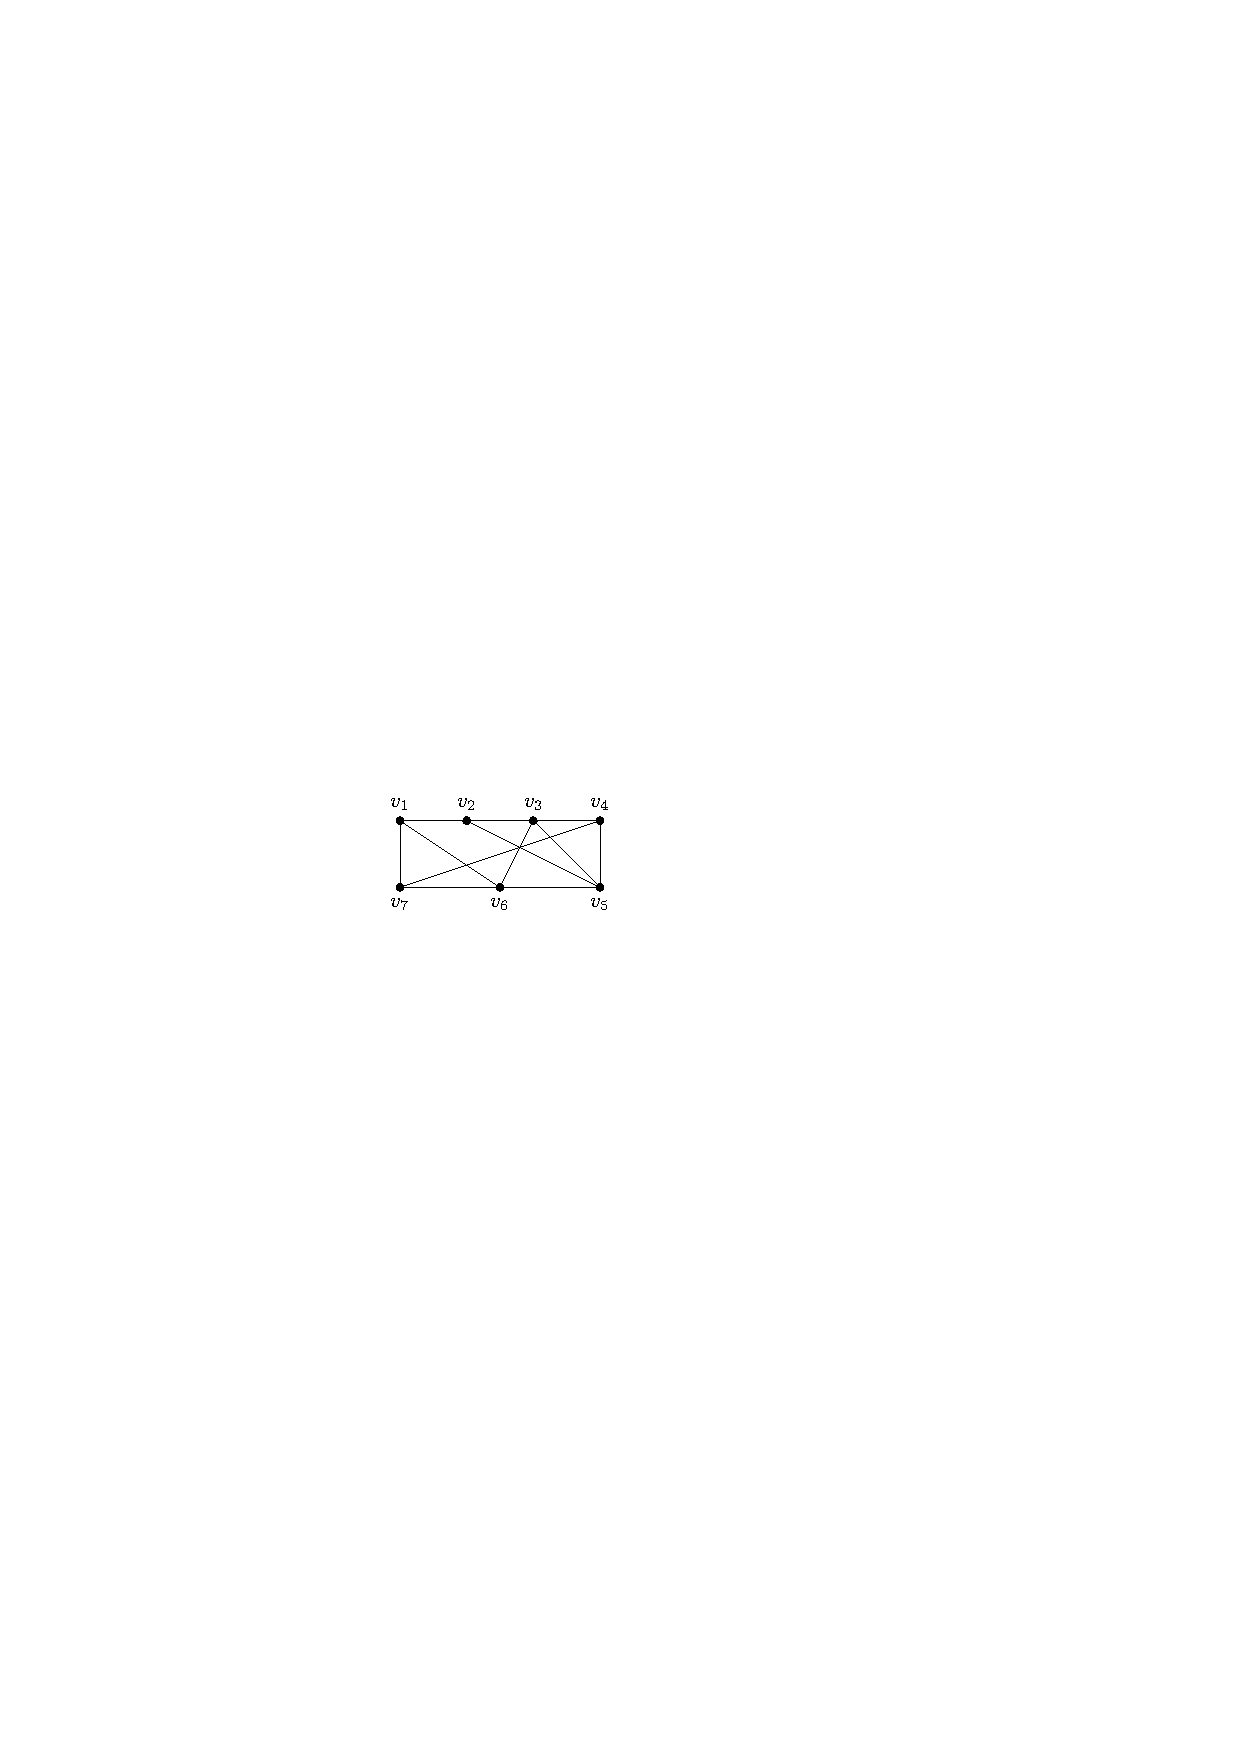
\includegraphics{Images/Subgraphs-G.pdf}} \hfill
\subcaptionbox{$H_1$\label{fig:SubgraphsH1}}{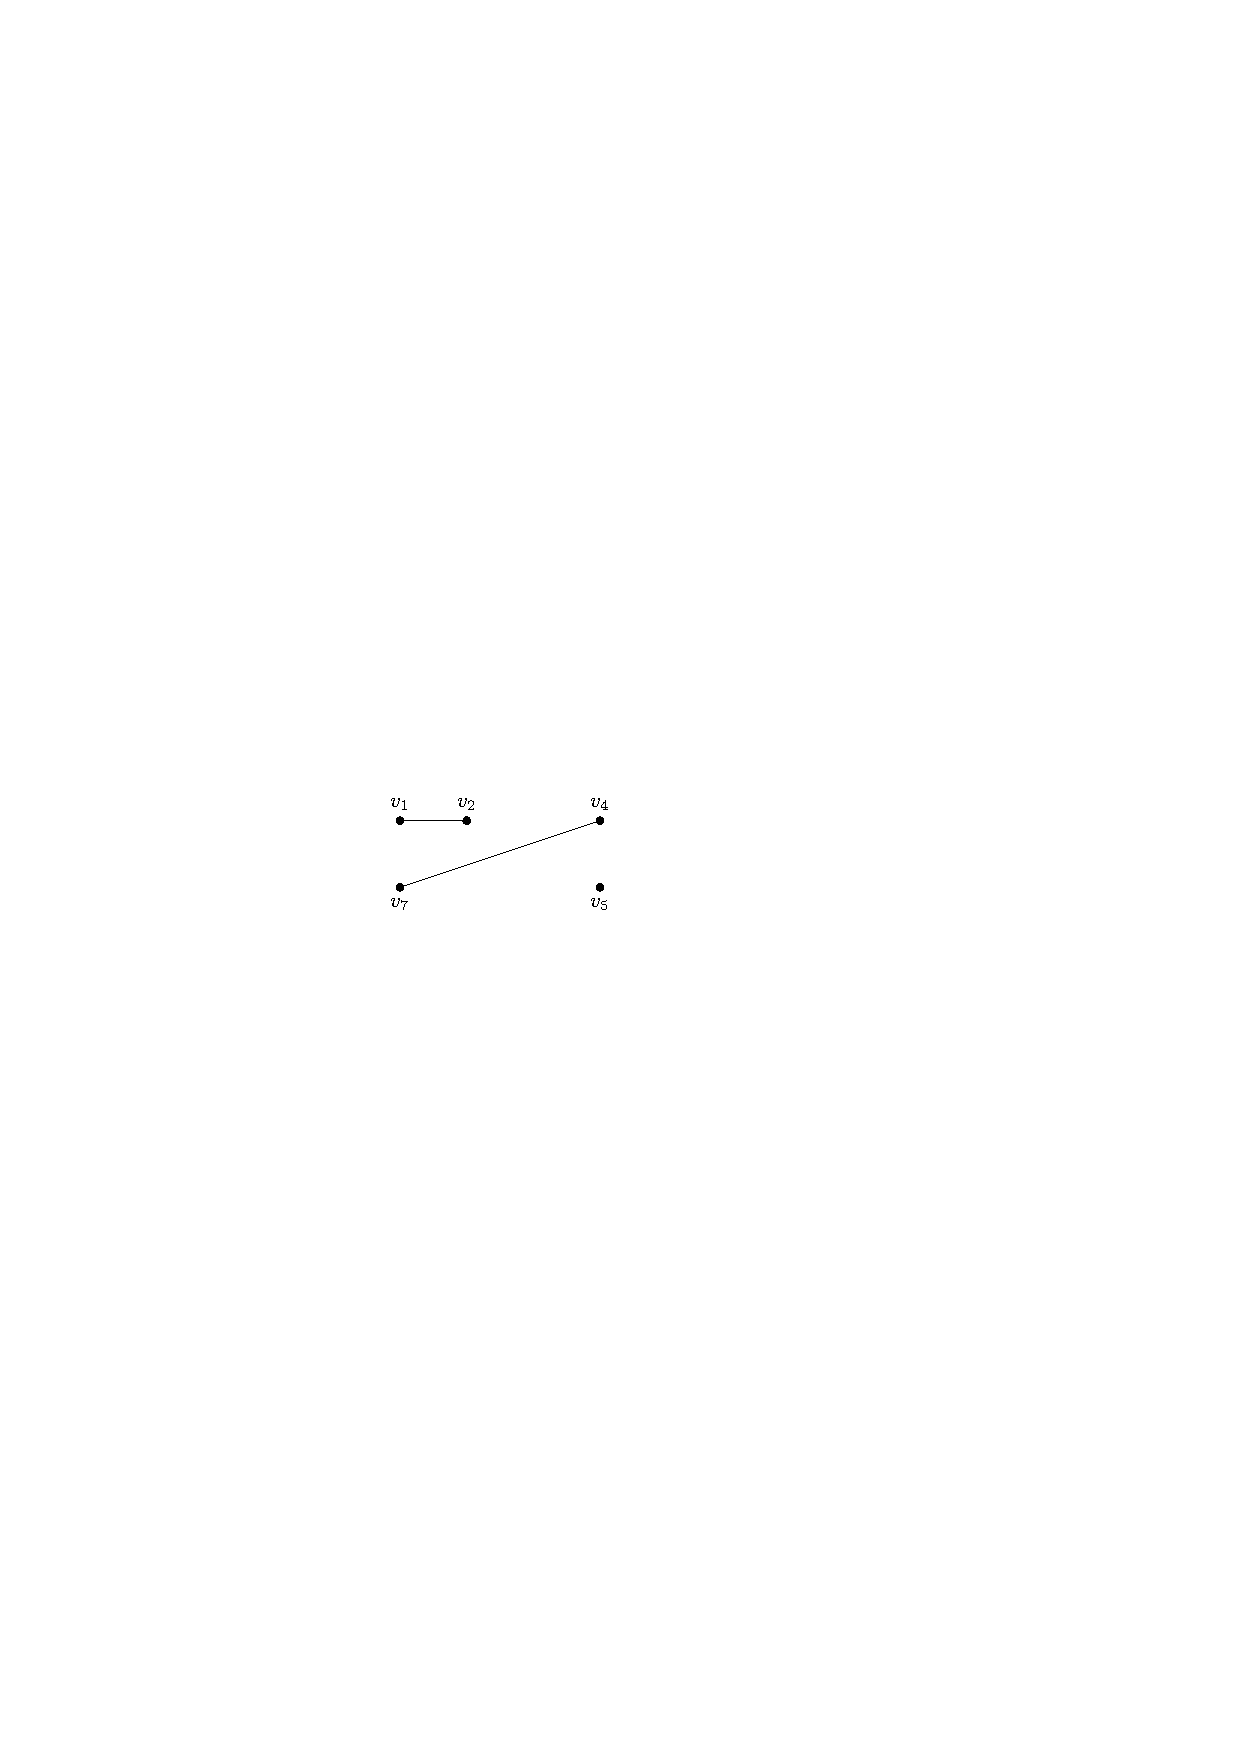
\includegraphics{Images/Subgraphs-H1.pdf}} \hfill
\subcaptionbox{$H_2$\label{fig:SubgraphsH2}}{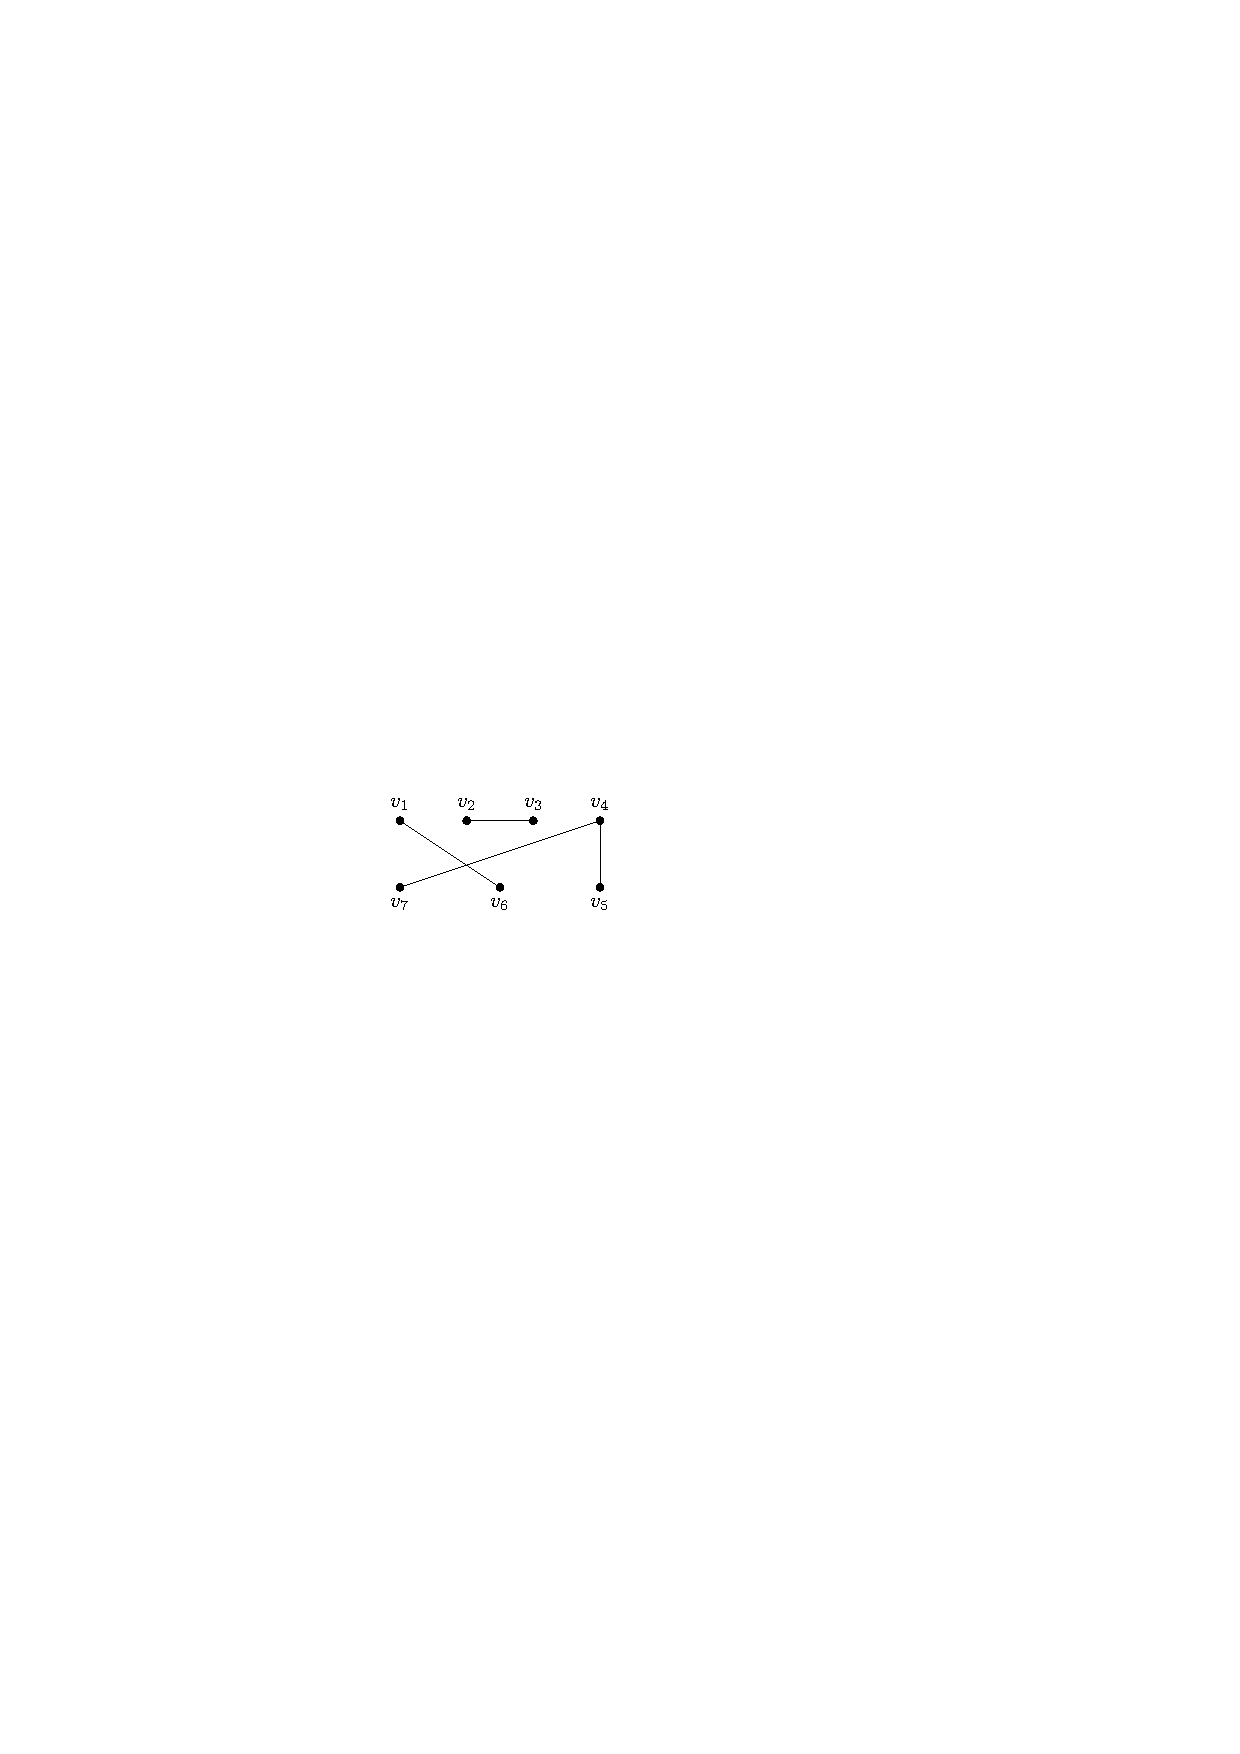
\includegraphics{Images/Subgraphs-H2.pdf}} \hfill
\subcaptionbox{$H_3$\label{fig:SubgraphsH3}}{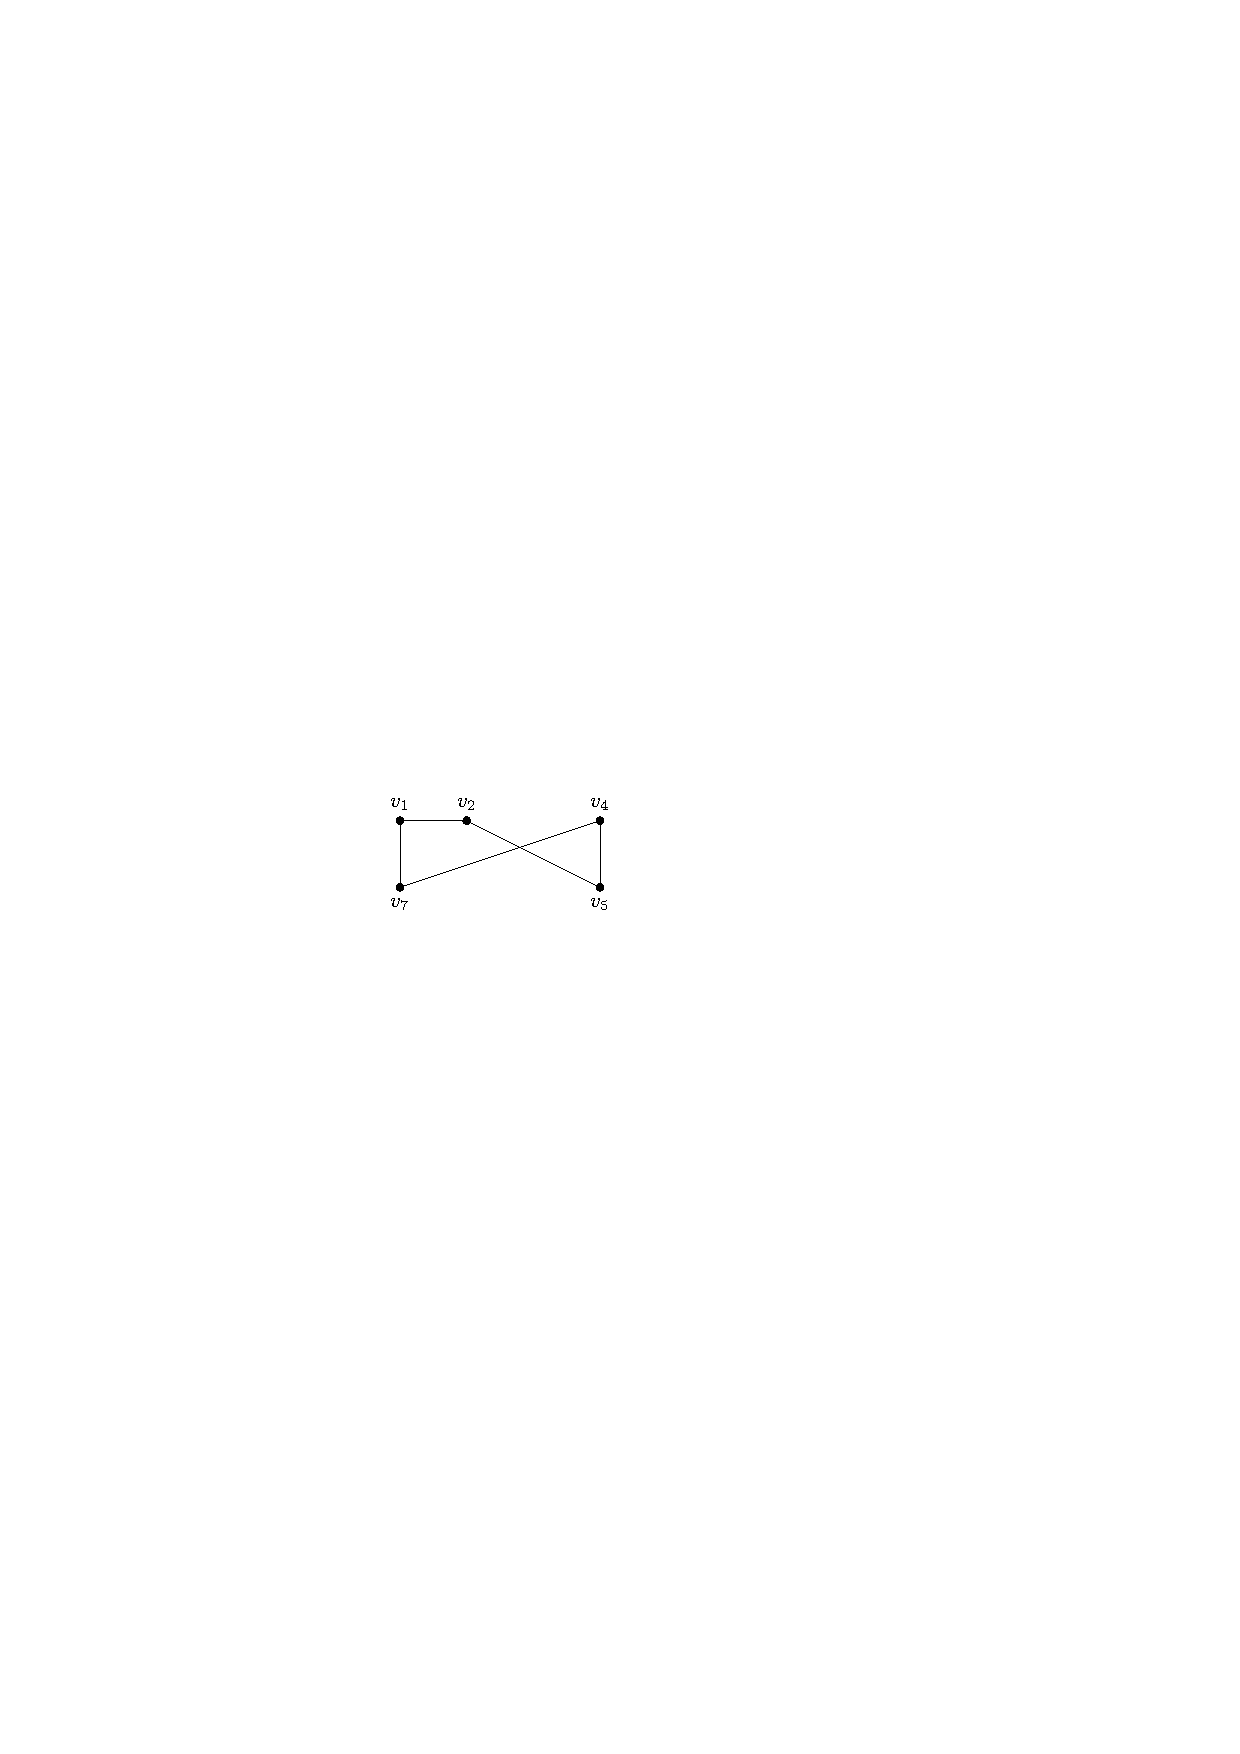
\includegraphics{Images/Subgraphs-H3.pdf}}
\caption{A graph with three of its subgraphs}\label{fig:Subgraphs}
\end{figure}
\end{Example}

A graph is \newterm{complete} if all its vertices are adjacent to one another. The complete graph of order $n$ is denoted by $K_n$. As there is an edge between every pair of distinct vertices of $K_n$, the size of $K_n$ is $\binom n 2$. The \newterm{totally disconnected graph} of order $n$, denoted by $\overline{K_n}$ is the graph of order $n$ that has no edges.

The \newterm{complement} of a graph $G$ is the graph $\overline G$ with the same vertices as $G$, in which any two vertices $u$ and $v$ are adjacent if and only if they are non-adjacent in $G$. Thus, if $G$ is an $(n, m)$-graph, then $\overline G$ is an $\pqty{n, \binom n 2 - m}$-graph. Observe that $\overline K_n$ is (as the notation suggests) the complement of $K_n$.

\begin{Exercise}
If $G$ is a graph of order $n$, and $\deg_G v = k$, what is $\deg_{\overline G} v$?
\end{Exercise}

\begin{Exercise}
Show that if $G$ and $\overline G$ are $k$-regular graphs of order $n$ then $k$ is an even number and $n = 4t + 1$ for some integer $t$.
\end{Exercise}

\subsection{Walks, Paths, and Cycles}\label{subsec:Walks}

A \newterm{walk} in a simple graph $G$ is a sequence of vertices $v_1, v_2, \ldots, v_k$ such that $v_i \sim v_{i + 1}$ for $i = 1, 2, \ldots, k - 1$. This is a walk \newterm{from $v_1$ to $v_k$} or \newterm{between $v_1$ and $v_k$}, having \newterm{length} $k - 1$. We may also say that this is a walk of length $k - 1$ starting at $v_1$ and ending at $v_k$.

A walk in which no vertex is repeated is a \newterm{path}. Note that the length of a path is the number of edges in it.

A \newterm{closed walk} in $G$ is a walk starting and ending at the same vertex. A closed walk in which no vertex is repeated (except for the start and end vertices being the same) is a \newterm{cycle}. The length of a cycle is also equal to the number of vertices in it. A cycle of the form $v_1, \ldots, v_{k-1}, v_k$ is usually referred to as ``the cycle $v_1, \ldots, v_{k-1}$''.

\begin{Example}\label{ex:Walk}
Consider the graph $G$ shown below.

\begin{center}
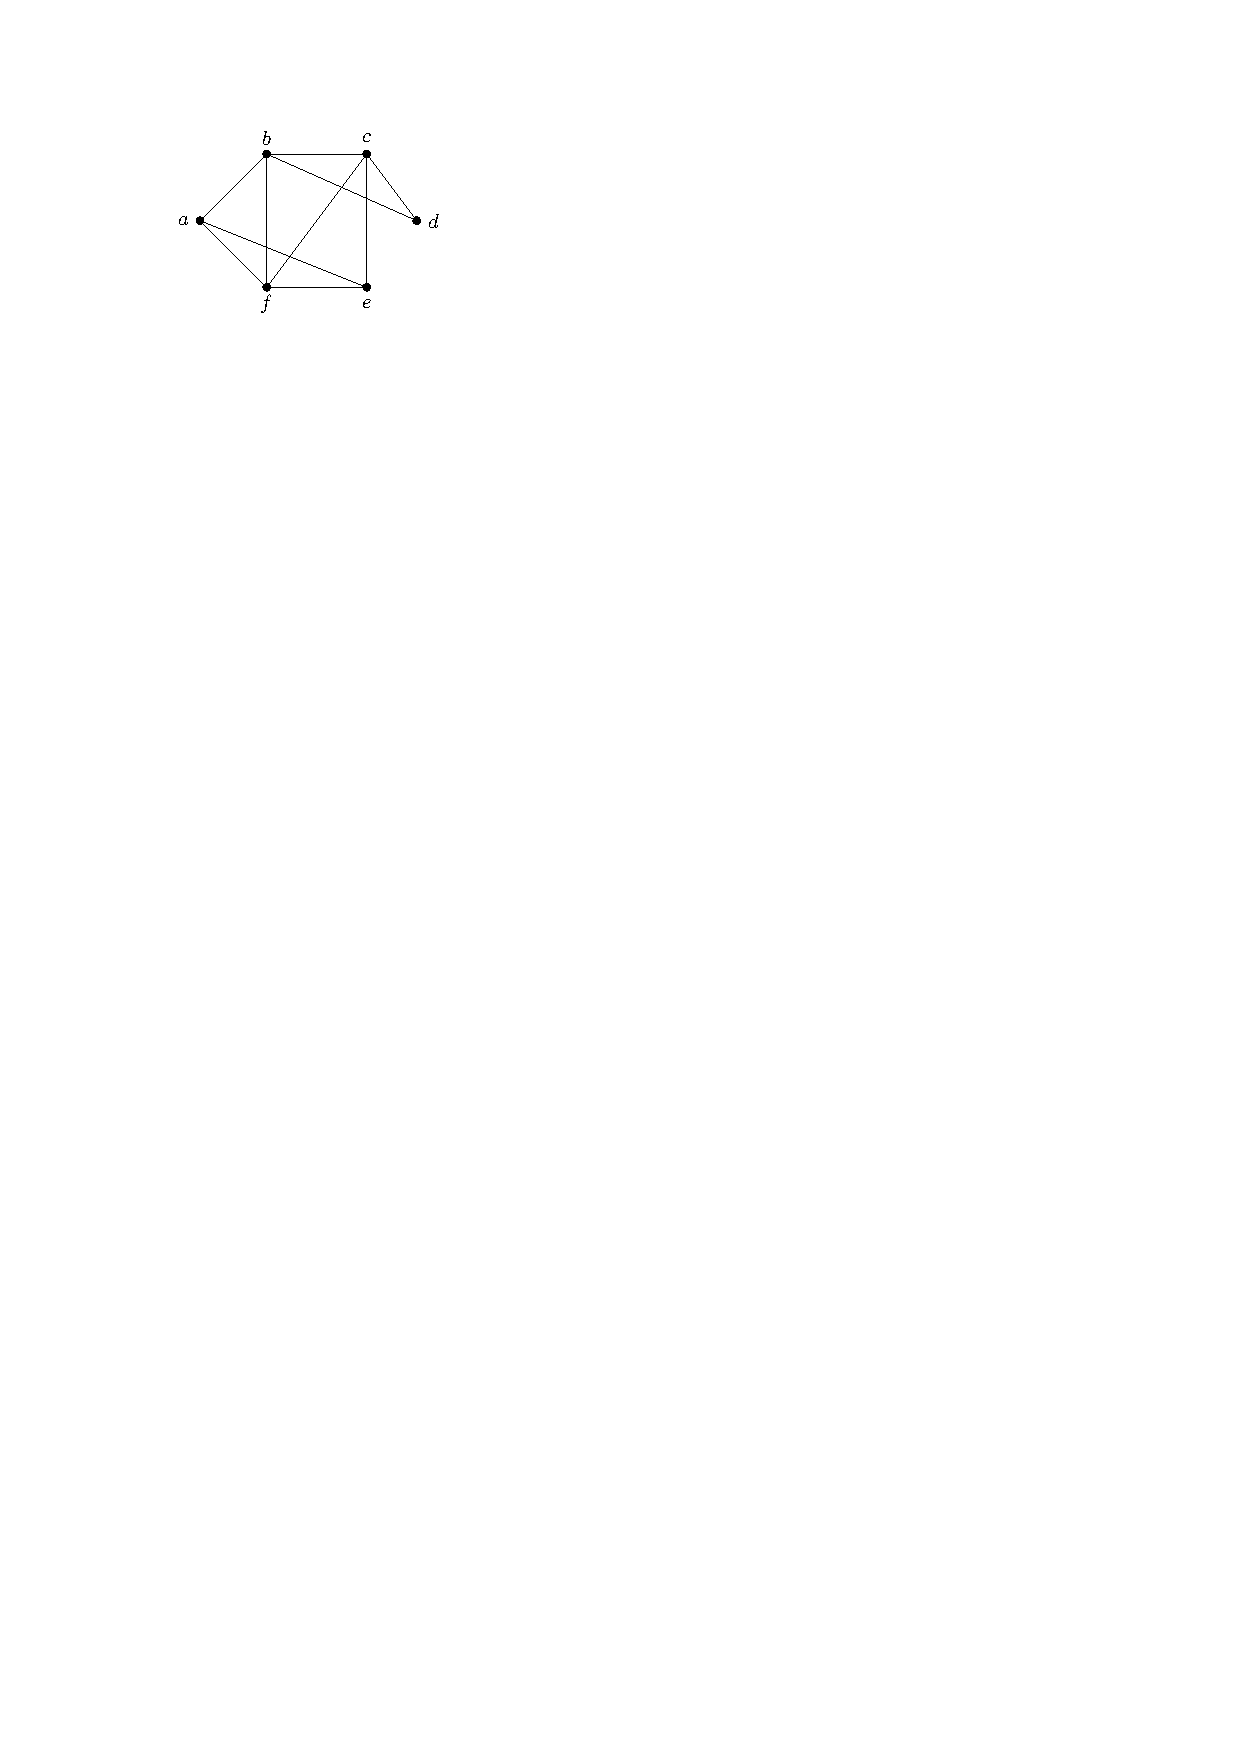
\includegraphics{Images/Walks.pdf}
\end{center}
A walk of length $5$ from $b$ to $c$ in $G$ is $b, f, e, a, e, c$.

\begin{center}
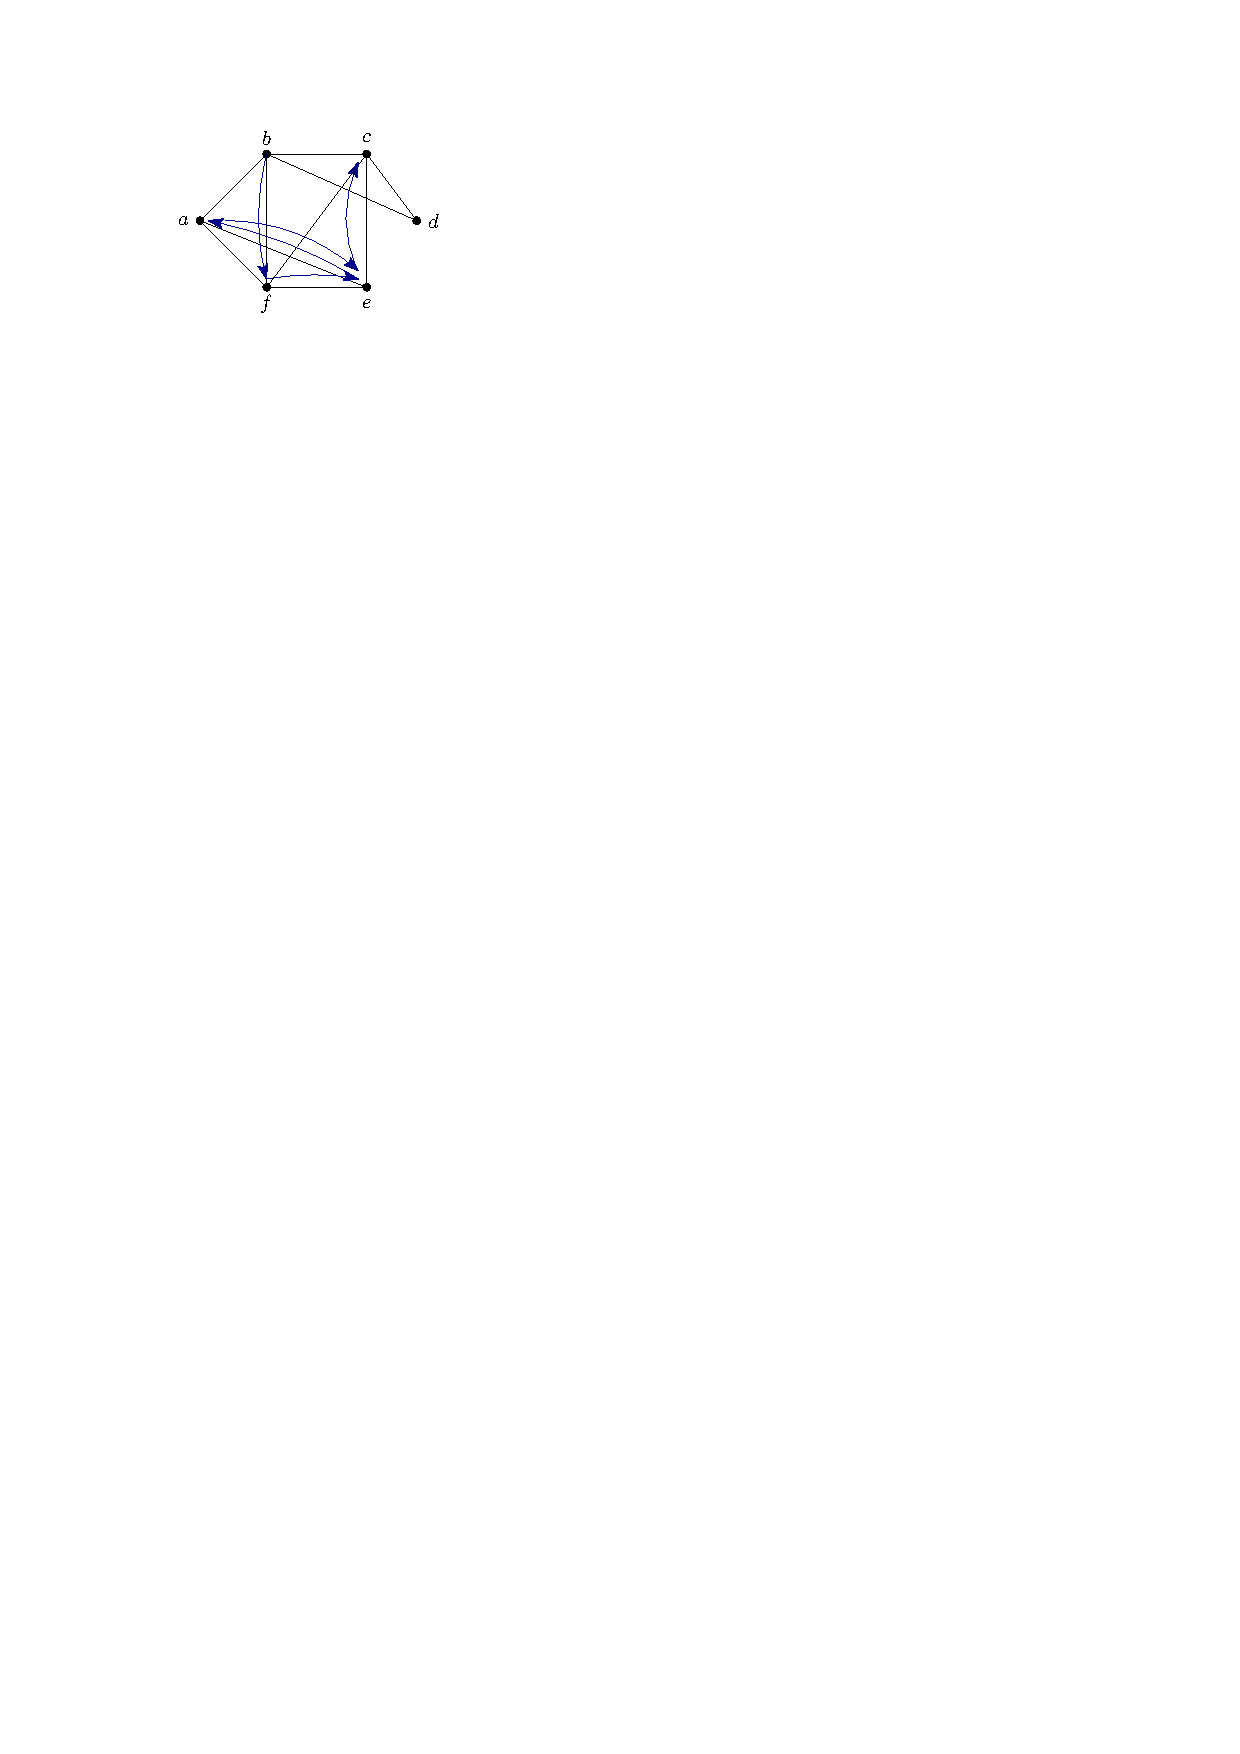
\includegraphics{Images/Walk1.pdf}
\end{center}
This walk is not a path, since the vertex $e$ is repeated. An example of a path from $b$ to $c$ in the same graph $G$ is $b, f, e, c$. The length of this path is $3$.

\begin{center}
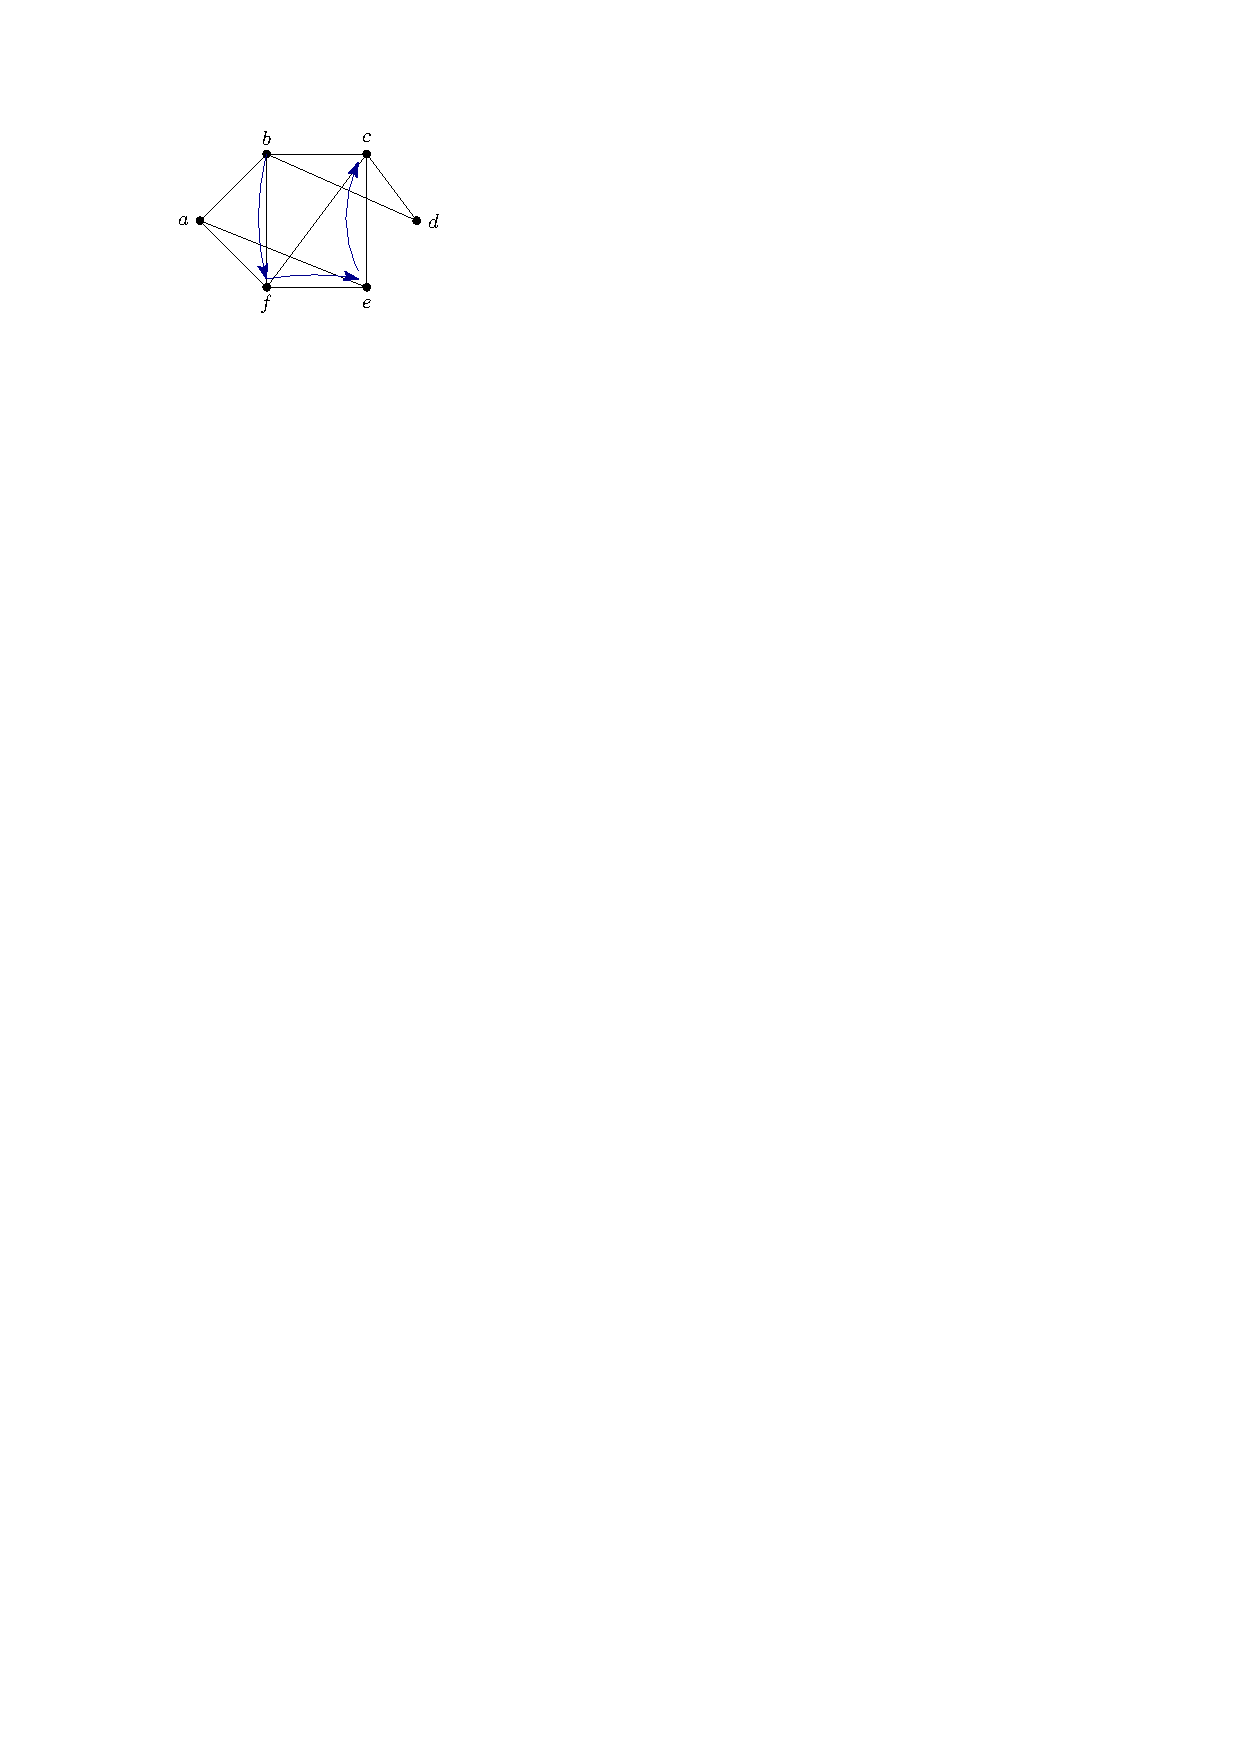
\includegraphics{Images/Path1.pdf}
\end{center}
A cycle of length $4$ in $G$ is $b, f, e, c, b$.

\begin{center}
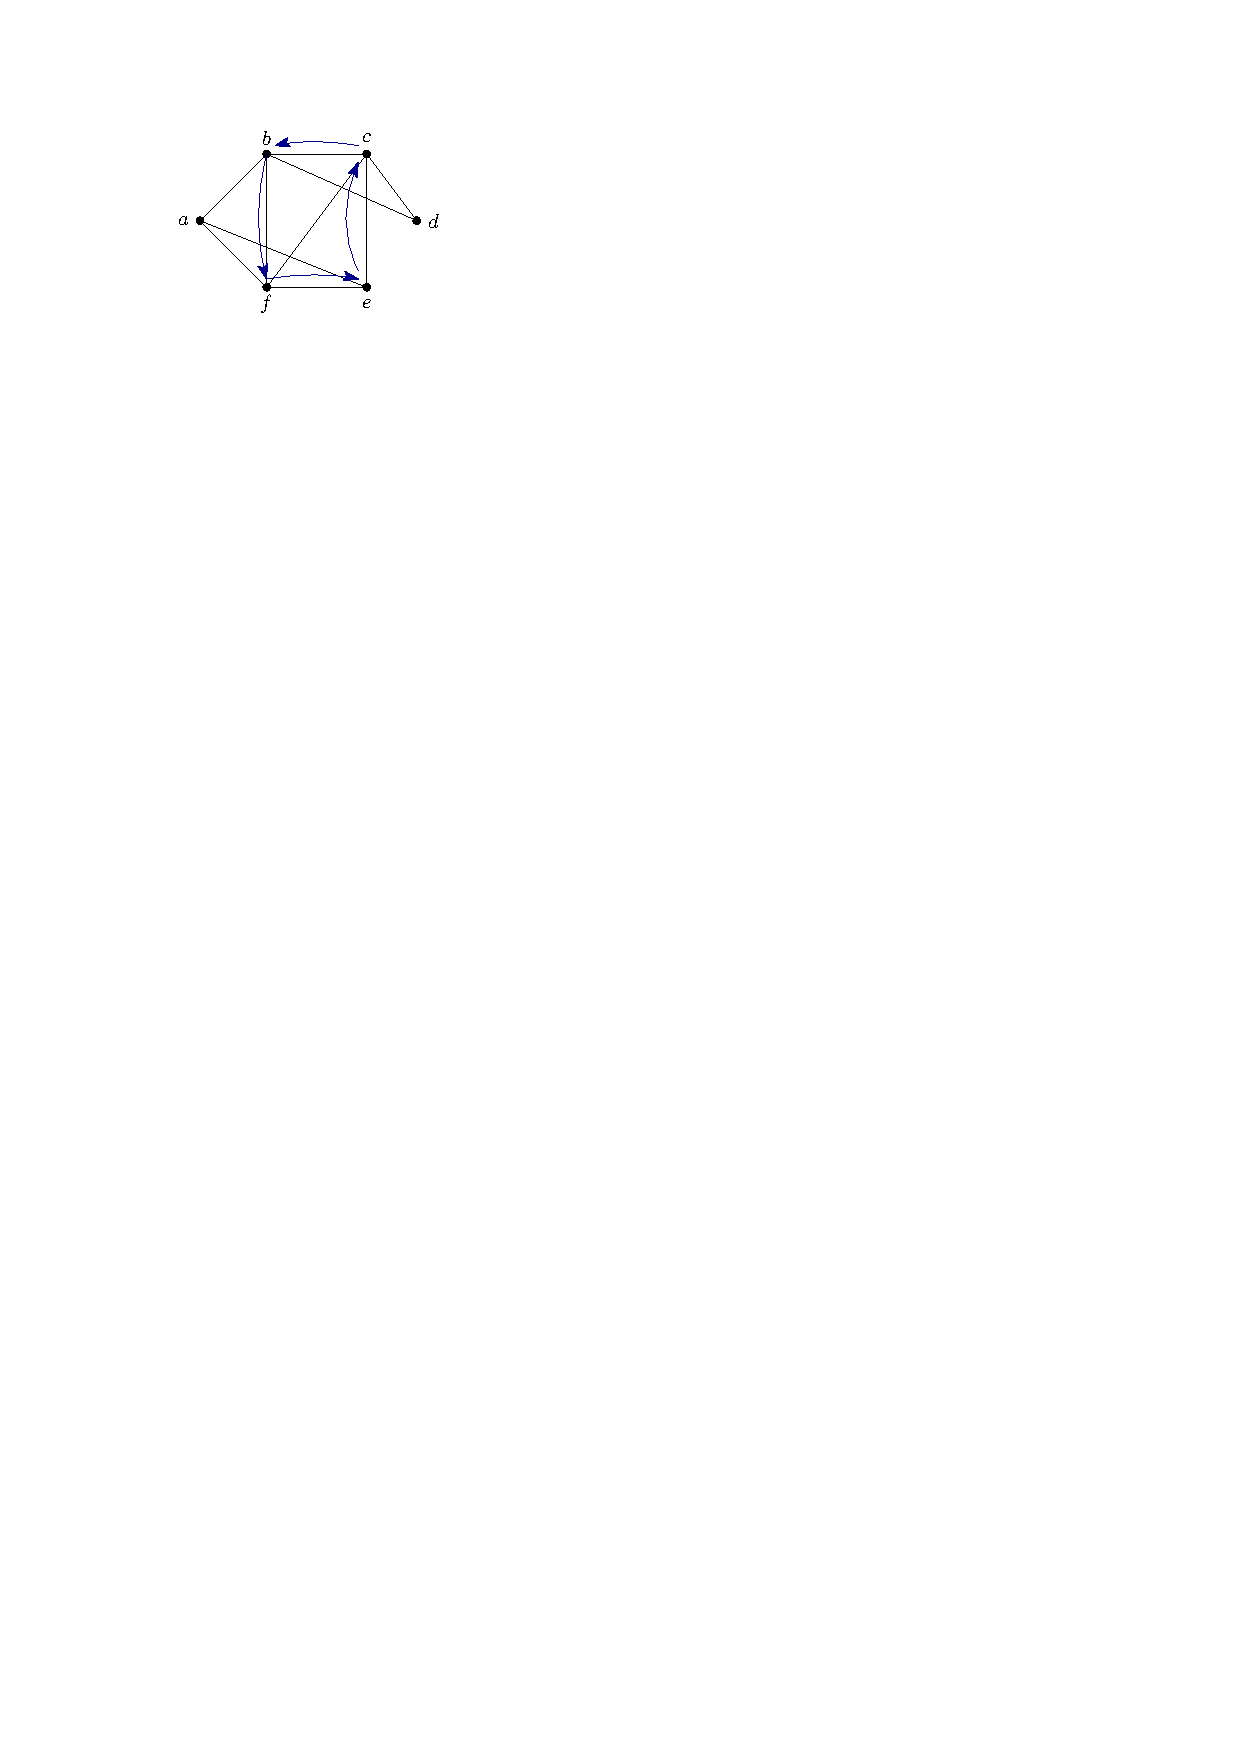
\includegraphics{Images/Cycle1.pdf}
\end{center}
\end{Example}

\subsection{Distances}\label{subsec:Distances}

The \newterm{distance} between two vertices $u$ and $v$ of a graph $G$ is the length of a shortest path between $u$ and $v$ -- such a shortest path between $u$ and $v$ is a \newterm{geodesic} from $u$ to $v$. Thus, the distance between $u$ and $v$ in $G$, denoted by $d_G(u, v)$ is the length of a geodesic from $u$ to $v$ in $G$. When the graph $G$ is clear from the context, we will write $d_G(u, v)$ as $d(u, v)$.

The \newterm{eccentricity} of a vertex $v$, denoted by $\ecc(v)$, is the maximum of the distances from $v$ to all the other vertices. That is,
\begin{equation*}
    \ecc(v) = \max_{u \in V(G)} d(u, v) .
\end{equation*}

The \newterm{diameter} of $G$ is the maximum of the eccentricities of vertices of $G$, and the \newterm{radius} of $G$ is the minimum of the eccentricities of vertices of $G$. They are denoted by $\diam(G)$ and $\rad(G)$ respectively. Thus,
\begin{align*}
    \diam(G) & = \max_{v \in V(G)} \ecc(v)= \max_{u, v \in V(G)} d(u, v) \\
    \rad(G) & = \min_{v \in V(G)}\ecc(v) = \min_{v \in V(G)} \max_{u \in V(G)} d(u, v).
\end{align*}

The set of all vertices of $G$ having minimum eccentricity, i.e.\ the set of all $v \in V(G)$ such that $\ecc v = \rad G$, is the \newterm{centre} of $G$.

\subsection{Connectedness}\label{subsec:Connectedness}

A graph is \newterm{connected} if there is a path between every two of its vertices. Otherwise, it is \newterm{disconnected}. A \newterm{(connected) component} of a graph $G$ is a maximal connected subgraph of $G$. Thus, a graph $G$ is connected if and only if it has exactly one component.

\begin{Theorem}\label{thm:GorGCompConn}
For any graph $G$, either $G$ or $\overline G$ is connected.
\end{Theorem}

\begin{proof}
Consider a graph $G$, and suppose that $G$ is disconnected. We shall show that $\overline G$ is connected, by showing that there is a path between every two vertices of $\overline G$.

Let $u$ and $v$ be any two vertices of $\overline G$. If they are not adjacent in $G$, then they are adjacent in $\overline G$, and hence there is a path $uv$ from $u$ to $v$ in $\overline G$. If $u$ and $v$ are adjacent in $G$, then they belong to the same component of $G$. As $G$ is disconnected, it has at least one more component containing at least one vertex, say $w$, which is necessarily non-adjacent to both $u$ and $v$. Hence, in $\overline G$, $w$ is adjacent to both $u$ and $v$. Thus, there is a path $uwv$ from $u$ to $v$ in $\overline G$. Therefore, $\overline G$ is connected.
\end{proof}

\begin{Theorem}\label{thm:Diam>=3}
For any connected graph $G$, if $\diam G \ge 3$, then $\diam \overline G \le 3$.
\end{Theorem}

\begin{proof}
Consider a graph $G$ of diameter at least $3$. Then there exist vertices $u$ and $v$ in $G$ such that $d_G(u, v) = 3$. This implies that $u$ and $v$ are non-adjacent in $G$, and hence adjacent in $\overline G$.

Now, consider any two vertices $x$ and $y$ other than $u$ and $v$. In $G$, $x$ can be adjacent to at most one of $u$ and $v$, for otherwise, $d_G(u,v) = 2$. Hence, $x$ is adjacent to at least one of $u$ and $v$ in $\overline G$. Similarly, $y$ is adjacent to at least one of $u$ and $v$ in $\overline G$. Thus, there is a path of length at most $3$ from $x$ to $y$ in $\overline G$ (namely $xuy$, $xvy$, $xuvy$, or $xvuy$), which implies that $d_{\overline G}(x, y) \le 3$. Therefore, $\diam \overline G \le 3$.
\end{proof}

\subsection{Graph Isomorphism}\label{subsec:Isomorphism}

An \newterm{isomorphism} from a graph $G$ to a graph $H$ is a bijective\footnote{injective and surjective; i.e.\ one-to-one and onto} function $f \colon V(G) \to V(H)$ such for all vertices $u$ and $v$ of $G$, $u \sim_G v$ if and only if $f(u) \sim_H f(v)$. In other words, a graph isomorphism is a bijection from the vertex set of the first graph to that of the second, that preserves both edges and non-edges. If there exists an isomorphism from $G$ to $H$, then $G$ and $H$ are \newterm{isomorphic}. Then we write $G \cong H$.

Isomorphic graphs have exactly the same structure -- i.e.\ all properties of the graph that do not depend on the labelling or drawing will be shared by isomorphic graphs. For example, isomorphic graphs have the same order, size, degree sequence, diameter, and radius. Indeed, if $f$ is an isomorphism from $G$ to $H$, and $v$ is a vertex of $G$, then the neighbours of $f(v)$ in $H$ are the images of the neighbours of $v$ in $G$, and $\deg_G v = \deg_H f(v)$. Similarly, if $u$ and $v$ are two vertices of $G$, then $d_G(u, v) = d_H(f(u), f(v))$.

\begin{Theorem}
Graph isomorphism is an equivalence relation on the class of all graphs.
\end{Theorem}

\begin{proof}
To show that graph isomorphism is an equivalence relation, we need to show that $\cong$ is a reflexive, symmetric, transitive relation between graphs. First, observe that the identity map on the vertex set of a graph is an isomorphism from the graph to itself -- for, if $G$ is a graph and $\id$ denotes the identity map on its vertex set then for any two vertices $u$ and $v$ of $G$, $u \sim v$ if and only if $\id(u) \sim \id(v)$, as $\id(u) = u$ and $\id(v) = v$. Hence, $\cong$ is reflexive.

Next, suppose that $G \cong H$. Then there exists an isomorphism $f$ from $G$ to $H$. Since $f \colon V(G) \to V(H)$ is bijective, it has an inverse $f^{-1} \colon V(H) \to V(G)$. We claim that $f^{-1}$ is an isomorphism from $H$ to $G$. We know that $f^{-1}$ is bijective. To see that it preserves edges and non-edges, observe that if $x$ and $y$ are two vertices of $H$, then $x = f(f^{-1}(x))$ and $y = f(f^{-1}(y))$, which implies that $x \sim_H y$ if and only if $f^{-1}(x) \sim_G f^{-1}(y)$ (since $f$ is an isomorphism from $G$ to $H$). Therefore, $f^{-1}$ is an isomorphism from $H$ to $G$. This shows that $H \cong G$. Thus, $\cong$ is symmetric.

Finally, suppose that $G \cong H$ and $H \cong K$. Then there exist isomorphisms $f$ from $G$ to $H$ and $g$ from $H$ to $K$. We claim that $g \circ f$ is an isomorphism from $G$ to $K$. Indeed, $g \circ f$ is a function from $V(G)$ to $V(K)$, and being a composition of bijections, is itself a bijection. Now, suppose $u$ and $v$ are two vertices of $G$. Then $u \sim_G v$ if and only if $f(u) \sim_H f(v)$ (since $f$ is an isomorphism from $G$ to $H$) if and only if $g(f(u)) \sim_K g(f(v))$ (since $g$ is an isomorphism from $H$ to $K$). Thus, $g \circ f$ is an isomorphism from $G$ to $K$. Therefore, $\cong$ is transitive.
\end{proof}

\subsection{Self-Complementary Graphs}\label{subsec:SC}

A graph is \newterm{self-complementary} if it is isomorphic to its complement -- i.e.\ $G$ is self-complementary if $G \cong \overline G$. For example, $K_1$, $P_4$ and $C_5$ are self-complementary graphs of orders $1$, $4$, and $5$ respectively. There is one more self-complementary graph of order $5$, namely the \newterm{bull graph}, which can be constructed by adding one new vertex to $P_4$ and making it adjacent to the two non-pendant vertices of the path. This graph is shown below.

\begin{center}
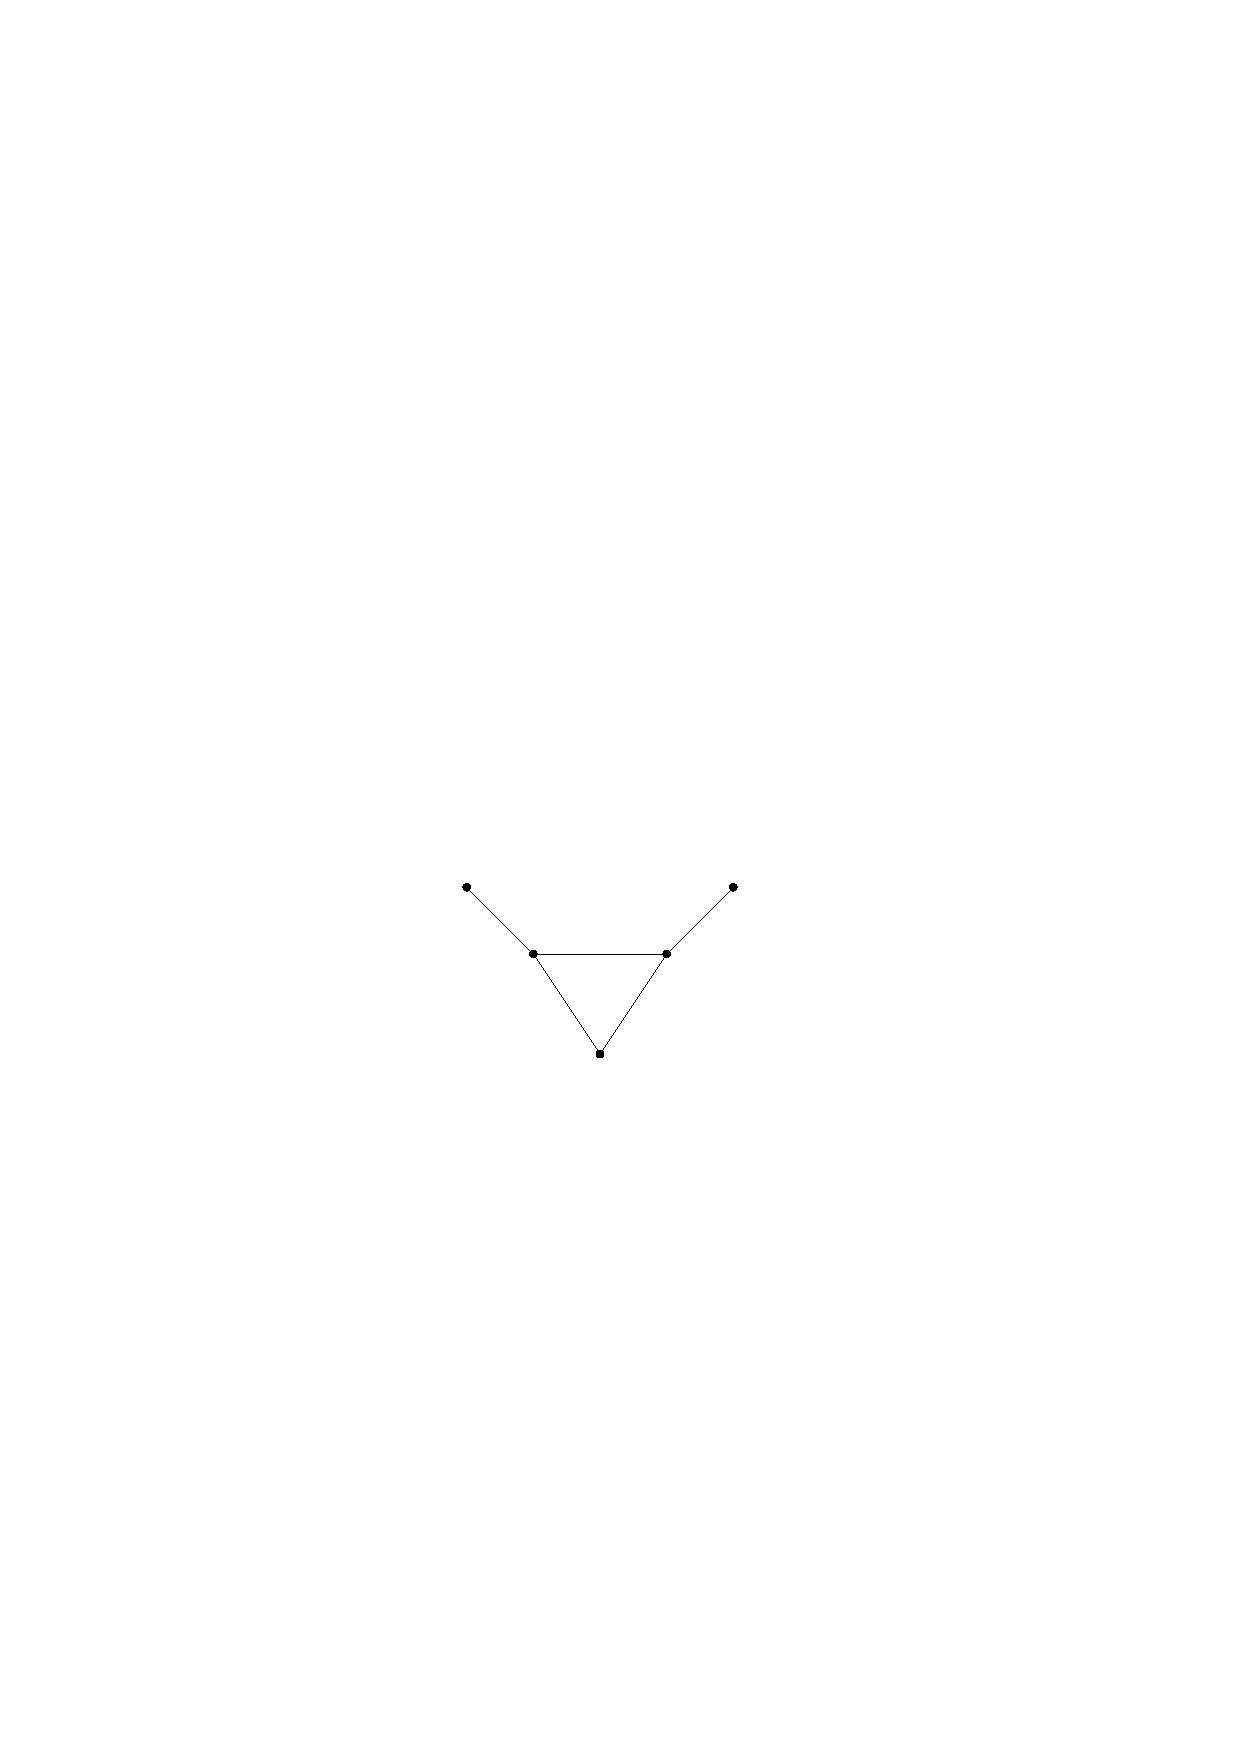
\includegraphics{Images/BullGraph.pdf}
\end{center}

\begin{Theorem}\label{thm:SCOrder}
The order of any self-complementary graph is $4k$ or $4k + 1$, for some non-negative integer $k$.
\end{Theorem}

\begin{proof}
Let $G$ be a self-complementary graph of order $n$ and size $m$. Then the size of $\overline G$ is $\binom n 2 - m$. Since $G \cong \overline G$, $m = \binom n 2 - m$, which implies that $m = \frac 1 2 \binom n 2 = \frac {n(n - 1)}{4}$. As $m$ is an integer, this implies that $4$ divides $n(n - 1)$, which in turn implies that either one of $n$ and $n - 1$ is divisible by $4$, or both $n$ and $n - 1$ are even. Since the latter is not possible, it follows that $n = 4k$ or $n - 1 = 4k$, i.e.\ $n = 4k$ or $4k + 1$ for some integer $k$.
\end{proof}


From \cref{thm:GorGCompConn}, we know that a graph and its complement cannot both be disconnected. Thus, if $G$ is a disconnected graph, then $\overline G$ must be connected, and therefore it cannot be isomorphic to $G$. This implies that a self-complementary graph is necessarily connected.

\begin{Corollary}\label{cor:SCConn}
Every self-complementary graph is connected. \qed
\end{Corollary}

Similarly, from \cref{thm:Diam>=3}, we obtain the following corollary about the diameter of self-complementary graphs.

\begin{Corollary}
Every non-trivial self-complementary graph has diameter $2$ or $3$.
\end{Corollary}

\begin{proof}
Consider a non-trivial, self-complementary graph $G$, and suppose that it has diameter strictly greater than $3$. Then, by \cref{thm:Diam>=3}, $\diam \overline G \le 3$, which implies that $\diam \overline G \ne \diam G$, a contradiction, since $G \cong \overline G$. Hence, $\diam G \le 3$. On the other hand, a non-trivial graph cannot have diameter $0$, hence $\diam G \ge 1$. But if $\diam G = 1$, then $G$ is a non-trivial complete graph, whose complement is a totally disconnected graph, which is again impossible. Hence, $\diam G = 2$ or $3$.
\end{proof}

\begin{Exercise}
If $G$ is a regular self-complementary graph of order $n$, show that $n = 4k + 1$, for some integer $k$, and $\diam G = 2$.
\end{Exercise}

\begin{Exercise}
Let $G$ be a self-complementary graph, and let $H$ be the graph obtained by taking the disjoint union of $H$ and $P_4$, and making every vertex of $H$ adjacent to the two non-pendant vertices of this $P_4$. Then show that $H$ is also self-complementary. What is the graph $H$ obtained in this manner if $G = K_1$?
\end{Exercise}

\begin{Exercise}
Construct a self-complementary graph of order $9$.
\end{Exercise}

\begin{Exercise}
Show that for each positive integer $n$ of the form $4k$ or $4k + 1$, where $k$ is an integer, there exists at least one self-complementary graph of order $n$.
\end{Exercise}

\subsection{Bipartite Graphs}\label{subsec:Bipartite}

A graph $G = (V, E)$ is \newterm{bipartite} if its vertex set $V$ can be partitioned into two subsets $V_1$ and $V_2$ such that no two vertices in $V_i$ are adjacent, for $i = 1, 2$. That is, there exist two non-empty, disjoint subsets $V_1, V_2 \subseteq V$ such that $V_1 \cup V_2 = V$, and every edge of $G$ (if any) joins a vertex in $V_1$ with a vertex in $V_2$. Then we say that $(V_1, V_2)$ is a \newterm{bipartition} of $G$.

The following theorem characterises bipartite graphs in terms of its cycles. A cycle is \newterm{even} if its length is even and \newterm{odd} if its length is odd.

\begin{Theorem}
A graph is bipartite if and only if it contains no odd cycles.
\end{Theorem}

\begin{proof}
First, suppose that $G$ is a bipartite graph with bipartition $(V_1, V_2)$, and let $v_1, v_2, \ldots, v_k$ be a cycle of length $k$ in $G$. Without loss of generality, suppose that $v_1 \in V_1$. Then, since $v_2 \sim v_1$, $v_2 \in V_2$, which in turn implies that $v_3 \in V_1$, as $v_2 \sim v_3$. Proceeding similarly, we see $v_i \in V_1$ if $i$ is odd and $v_i \in V_2$ if $i$ is even. But $v_k \sim v_1$ and $v_1 \in V_1$ implies that $v_k \in V_2$. Therefore, $k$ (the length of the cycle) is even.

Conversely, suppose $G$ is a graph that has no odd cycles. Without loss of generality, assume that $G$ is connected -- otherwise, apply the argument to each component. Let $v$ be any vertex of $G$. Define subsets $V_1$ and $V_2$ of $V(G)$ as follows:
\begin{align*}
    V_1 = \qty{\, u \in V \mid d(u, v)\ \text{is even} \,} \\
    V_2 = \qty{\, u \in V \mid d(u, v)\ \text{is odd} \,}.
\end{align*}
We claim that $(V_1, V_2)$ is a bipartition of $G$.

Suppose not, and let $x$ and $y$ be adjacent vertices of $G$, both belonging to $V_i$ for $i = 1$ or $2$. Let $P$ and $Q$ be shortest paths from $v$ to $x$ and $y$ respectively. Let $w$ be the last vertex common to both $P$ and $Q$ when traversing $P$ from $v$ to $x$. Then the portion of $P$ from $w$ to $x$, the edge $(x, y)$, and the portion of $Q$ from $y$ to $w$ forms a cycle in $G$, having length, say $l$, given by
\begin{align*}
l & = d(w, x) + d(w, y) + 1 \\
& = [d(v, x) - d(v, w)] + [d(v, y) - d(v, w)] + 1 \\
& = d(v, x) + d(v, y) - 2 d(v, w) + 1.
\end{align*}
If $x, y \in V_1$, then both $d(v, x)$ and $d(v, y)$ are even, and if $x, y \in V_2$, then both these numbers are odd. In either case, $d(v, x) + d(v, y)$ is even, and hence $l$ is odd, which is a contradiction. Hence, $(V_1, V_2)$ is a bipartition of $G$ as claimed.
\end{proof}

\subsection{Trees}\label{subsec:Trees}

A \newterm{tree} is a connected, acyclic graph. There are several well known characterisations or alternative definitions of trees. We take the given definition as the basic one and prove its equivalence to some others.

\begin{Theorem}\label{thm:UniPath}
A graph $T$ is a tree if and only if there is a unique path joining every two vertices of $T$.
\end{Theorem}
\begin{proof}
First, suppose that $T$ is a tree, and let $u$ and $v$ be vertices of $T$. Since $T$ is connected, there is a path, say $P_1$, joining $u$ and $v$. Now we must show that this path is unique. Assume to the contrary that there exists another path $P_2$ from $u$ to $v$. When traversing $P_1$ from $u$ to $v$, let $w$ be the first vertex that is present on $P_1$ but not $P_2$. Let $x$ be the vertex on $P_1$ preceding $w$, and note that $x$ is on $P_2$ as well. Let $y$ be the next vertex common to both $P_1$ and $P_2$ when traversing $P_1$ from $x$ to $v$. Then the portion of $P_1$ from $x$ to $y$ together with the portion of $P_2$ from $y$ to $x$ forms a cycle in the tree $T$, which is a contradiction. Thus, $P_1$ is the unique path joining $u$ and $v$.

Conversely, suppose that $T$ is a graph in which there is a unique path joining any two vertices. Clearly, $T$ is connected. To show that $T$ is acyclic, suppose that $v_1, v_2, \ldots, v_n$ is a cycle in $T$. Then we get two different paths joining $v_1$ and $v_n$, namely the path $v_1, v_2, \ldots, v_n$ and the path $v_1, v_n$ (since $v_1 \sim v_n$ in the cycle). This contradicts our assumption. Thus, $T$ must be acyclic and hence, is a tree.
\end{proof}

The next two results show that the size of a tree is always one less than its order, and that conversely, this property together with either connectedness or acyclicity implies that the graph is a tree.
\begin{Theorem}\label{thm:Conn;p=q+1}
A $(p, q)$-graph $T$ is a tree if and only if it is connected and $p = q + 1$.
\end{Theorem}
\begin{proof}
Let $T$ be a tree with $p$ vertices and $q$ edges. Then $T$ is connected. We prove that $p = q + 1$ by induction. This is clearly true when $p = 1$. Assume it to be true for all trees of order less than $p$. Now in $T$, we know that every two vertices are joined by a unique path. Thus, if $e$ is any edge of $T$, then the graph $T - \{e\}$ obtained by deleting $e$ has exactly two components, say $T_1$ and $T_2$. Each one is a tree, since it is connected and acyclic. Let $T_i$ have $p_i$ vertices and $q_i$ edges, $i = 1, 2$. Then by the hypothesis, $p_i = q_i + 1$ (since $p_i < p$). But $p = p_1 + p_2$ and $q = q_1 + q_2 + 1$ (since the size of $T - \{e\}$ is one less than that of $T$). Thus, $p = q_1 + q_2 + 2 = q + 1$.

For the converse, suppose that $T$ is a connected $(p,q)$-graph with $p = q + 1$. We must show that is acyclic. Suppose to the contrary that $T$ has a cycle $C$ with $k$ vertices. Then $C$ has $k$ edges as well. Since $T$ is connected, there is a path from every vertex not on $C$ to some vertex of $C$. The shortest path from each vertex $v$ not on $C$ to a vertex on $C$ has a unique edge incident with $v$, which is not part of $C$. Since there are $p - k$ vertices in $T$ not on $C$, there are $p - k$ such edges. Thus $q \ge (p - k) + k = p$, which contradicts our assumption that $p = q + 1$. Thus, $T$ must be acyclic.
\end{proof}

In the following theorem, the proof of the direct part is identical to that of Theorem~\ref{thm:Conn;p=q+1}, except for the assertion being about acyclicity rather than connectedness. The proof of the converse part is entirely different.
\begin{Theorem}\label{thm:Acyc;p=q+1}
A $(p,q)$-graph $T$ is a tree if and only if it is acyclic and $p = q + 1$.
\end{Theorem}
\begin{proof}
Let $T$ be a tree with $p$ vertices and $q$ edges. Then $T$ is acyclic. We prove that $p = q + 1$ by induction. This is clearly true when $p = 1$. Assume it to be true for all trees of order less than $p$. Now in $T$, we know that every two vertices are joined by a unique path. Thus, if $e$ is any edge of $T$, then the graph $T - \{e\}$ obtained by deleting $e$ has exactly two components, say $T_1$ and $T_2$. Each one is a tree, since it is connected and acyclic. Let $T_i$ have $p_i$ vertices and $q_i$ edges, $i = 1, 2$. Then by the hypothesis, $p_i = q_i + 1$ (since $p_i < p$). But $p = p_1 + p_2$ and $q = q_1 + q_2 + 1$ (since the size of $T - \{e\}$ is one less than that of $T$). Thus, $p = q_1 + q_2 + 2 = q + 1$.

Conversely, suppose that $T$ is an acyclic $(p,q)$-graph with $p = q + 1$. To show that $T$ is connected, we need to prove that it is connected -- i.e.\ it has only one component. Let $T$ have $k$ components $T_1, \ldots, T_k$. Each one is acyclic, and being connected, is a tree. Thus from the first part of the theorem, we know that if $p_i$ and $q_i$ are respectively the order and size of the component $T_i$, $p_i = q_i + 1$. Now $p = p_1 + \cdots p_k = (q_1 + 1) + \cdots + (q_k + 1) = q + k$. But we know that $p = q + 1$. Therefore, $k = 1$. Thus, $T$ is a tree.
\end{proof}

\begin{Exercise}\label{exer:TreePendantVertices}
A \newterm{pendant vertex} of a graph is a vertex of degree $1$. Prove that every non-trivial tree contains at least two pendant vertices. \\
\hint{TreePendantVertices}{Observe that a non-trivial tree cannot have a vertex of degree zero. Use Handshaking Lemma and assume every degree is at least $2$ to get a contradiction.}
\end{Exercise}

\begin{Exercise}\label{exer:TreeCentre}
The \newterm{centre} of a graph $G$ is the set of all vertices of $G$ with minimum eccentricity -- i.e.\ the set of all vertices $v$ of $G$ with $\ecc v = \rad v$. Show that every tree has a centre consisting of either exactly one vertex or exactly two adjacent vertices.\\
\hint{TreeCentre}{Observe that deleting all pendant vertices of a tree results in a new tree with the same centre.}
\end{Exercise}

\solution{TreeCentre}{
Let $T$ be a tree on $n$ vertices. We prove the result by induction on $n$.

If $n = 1$ or $2$, the result obviously holds. Suppose, for the sake of induction, that the result holds for all trees of order less than $n$.

Consider $T$, of order $n \ge 3$. Then $T$ has at least two pendant vertices. Let $T'$ be the tree (of order less than $n$) obtained by deleting all the pendant vertices of $T$.

Then the vertices of $T'$ have eccentricities exactly one less than their eccentricities in $T$, and therefore, $T$ and $T'$ have the same centre. Hence, the result follows by induction.
}

\subsection{Adjacency Matrices}\label{subsec:AdjMat}

The \newterm{adjacency matrix} of a graph $G$ of order $n$, with vertex set $V = \{v_1, \ldots, v_n\}$, is the $n \times n$ matrix $A = \mathcal A(G)$ whose $(i,j)$-entry is
\begin{equation*}
a_{ij} = \begin{cases}
1, & v_i \sim v_j \\
0, & v_i \nsim v_j.
\end{cases}
\end{equation*}

\begin{Example}\label{ex:GNM(6-11)AdjMat}
The adjacency matrix of the graph
\begin{center}
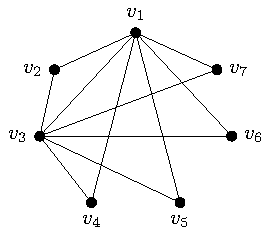
\includegraphics{Images/GNM(6,11).pdf}
\end{center}
is
\begin{equation*}
A = \begin{bmatrix}
0 & 1 & 1 & 1 & 1 & 1 & 1 \\
1 & 0 & 1 & 0 & 0 & 0 & 0 \\
1 & 1 & 0 & 1 & 1 & 1 & 1 \\
1 & 0 & 1 & 0 & 0 & 0 & 0 \\
1 & 0 & 1 & 0 & 0 & 0 & 0 \\
1 & 0 & 1 & 0 & 0 & 0 & 0 \\
1 & 0 & 1 & 0 & 0 & 0 & 0
\end{bmatrix}.
\end{equation*}
\end{Example}

Observe that, as the graphs we discuss are simple graphs and therefore have no self-loops on vertices, no vertex is adjacent to itself -- i.e.\ $a_{ii} = 0$ for all $i = 1, \ldots, n$. Also, since the graphs are undirected, $v_i \sim v_j$ if and only if $v_j \sim v_i$ -- i.e.\ $a_{ij} = a_{ji}$. Thus, we have the following observation.

\begin{Observation}
The adjacency matrix of a (simple, undirected) graph is a symmetric, zero-diagonal, $(0, 1)$-matrix.
\end{Observation}

In the $i$\nth row of the adjacency matrix, for each $j$, the $j$\nth entry is $1$ if $v_j$ is adjacent to $v_i$, and $0$ otherwise. That is, the number of $1$s in the $i$\nth row is the number of vertices adjacent to $v_i$, or in other words, the degree of $v_i$. Thus, the row sums of $A$ are the vertex degrees. Observe that $A \mathbbm 1$ is the vector of row sums, where $\mathbbm 1$ is the vector (of suitable size) with all entries equal to $1$. For instance, with the matrix $A$ given in \cref{ex:GNM(6-11)AdjMat},
\begin{equation*}
A = \begin{bmatrix}
0 & 1 & 1 & 1 & 1 & 1 & 1 \\
1 & 0 & 1 & 0 & 0 & 0 & 0 \\
1 & 1 & 0 & 1 & 1 & 1 & 1 \\
1 & 0 & 1 & 0 & 0 & 0 & 0 \\
1 & 0 & 1 & 0 & 0 & 0 & 0 \\
1 & 0 & 1 & 0 & 0 & 0 & 0 \\
1 & 0 & 1 & 0 & 0 & 0 & 0
\end{bmatrix}
\begin{bmatrix}
1 \\ 1 \\ 1 \\ 1 \\ 1 \\ 1 \\ 1
\end{bmatrix} =
\begin{bmatrix}
6 \\ 2 \\ 6 \\ 2 \\ 2 \\ 2 \\ 2
\end{bmatrix}.
\end{equation*}
From the Handshaking Lemma and the preceding observation, it follows that the sum of all entries of $A$ is twice the number of edges of the graph.

\begin{Exercise}
Show that for any graph $G$ of order $n$, $\mathcal A(\overline G) = J - I - \mathcal A(G)$ where $I$ is the identity matrix and $J$ is the square all-ones matrix (i.e.\ a matrix with all entries $1$), both of order $n$.
\end{Exercise}

\begin{Exercise}
Suppose $G$ is a disconnected graph with components $G_1, G_2, \ldots, G_k$, and furthermore, assume that the vertices are ordered in such a way that the first $n_1$ vertices are in $G_1$, the next $n_2$ vertices are in $G_2$, and so on, the last $n_k$ vertices are in $G_k$. Show that the adjacency matrix of $G$ is given by the partitioned matrix
\begin{equation*}
\mathcal A(G) = \begin{bmatrix}
\mathcal A(G_1) & 0_{n_2} & \cdots & 0_{n_k} \\
0_{n_1} & \mathcal A(G_2) & \cdots & 0_{n_k} \\
\vdots & \vdots & \ddots & \vdots \\
0_{n_1} & 0_{n_k} & \cdots & \mathcal A(G_k)
\end{bmatrix}
\end{equation*}
where $0_{n_i}$ denotes the $n_i \times n_i$ zero-matrix.
\end{Exercise}

\begin{Exercise}\label{exer:A2ij}
Show that the $(i,j)$-entry of $A^2$ is the number of walks of length $2$ from $v_i$ to $v_j$. Hence show that $\trace(A^2) = 2|E(G)|$.\\
\hint{A2ij}{Recall that if $A$ is any $n \times n$ matrix, then the $(i,j)$-entry of $A^2$ is $\sum_{k=1}^{n} a_{ik}a_{kj}$. As $A$ is a $(0, 1)$-matrix, each term in this summation is $1$ or $0$, with the former if and only if $a_{ik} = a_{kj} = 1$. What does this imply about the vertices $v_i$, $v_k$, and $v_j$? Then, as $k$ varies from $1$ to $n$, what does the value of the sum imply about $v_i$ and $v_j$?}
\end{Exercise}

The following result (which generalises the statement in \cref{exer:A2ij}) shows that the adjacency matrix can be used to obtain certain information about walks in the graph.

\begin{Theorem}
Let $A$ be the adjacency matrix of a graph $G$ with vertex set $\{v_1, \ldots, v_n\}$. Then the $(i,j)$-entry of $A^m$, for any positive integer $m$, is the number of walks of length $m$ from $v_i$ to $v_j$.
\end{Theorem}

\begin{proof}
We prove the result by induction on $m$. For $m = 1$, the $(i,j)$-entry of $A^1 = A$ is $a_{ij}$, which is $1$ if and only if $v_i$ is adjacent to $v_j$, i.e.\ if and only if there is a walk of length $1$ (namely, an edge) from $v_i$ to $v_j$. Thus, the result holds for $m = 1$.

Now suppose, for the sake of induction, that the result holds for some $m \ge 1$, and consider $A^{m + 1}$. The $(i,j)$-entry of $A^{m + 1}$ is
\begin{equation*}
(A^{m + 1})_{ij} = \sum_{k = 1}^{n} (A^m)_{ik} a_{kj}.
\end{equation*}
First, note that $a_{kj} = 1$ if and only if $v_k \sim v_j$. Therefore, the above sum is equal to the sum of all $(A^m)_{ik}$ where $v_k \sim v_j$. Now, by the induction hypothesis, $(A^m)_{ik}$ is the number of walks of length $m$ from $v_i$ to $v_k$. If $v_j$ is adjacent to $v_j$, then each walk of length $m$ from $v_i$ to $v_k$, together with the edge from $v_j$ to $v_j$, forms a walk of length $m + 1$ from $v_i$ to $v_j$. Thus, for each $k$ such that $v_k \sim v_j$, $(A^m)_{ik} a_{kj} = (A^m)_{ik}$ is the number of walks of length $m + 1$ from $v_i$ to $v_j$ that pass through $k$. Summing over all $k$, this gives the total number of walks of length $m + 1$ from $v_i$ to $v_j$. Hence the result follows by induction.
\end{proof}

Alternatively, note that
\begin{equation*}
(A^m)_{ij} = \sum_{k_1, k_2, \ldots, k_{m-1}} a_{i k_1} a_{k_1 k_2} \cdots a_{k_{m-1} j}
\end{equation*}
and each term in this summation will be $1$ if and only if $a_{i k_1} = a_{k_1 k_2} = \cdots = a_{k_{m-1} j} = 1$, i.e.\ $v_i \sim v_{k_1} \sim v_{k_2} \sim \cdots \sim v_{k_{m-1}} \sim v_j$, which corresponds to a walk of length $m$ from $v_i$ to $v_j$. Hence $(A^m)_{ij}$ is the number of walks of length $m$ from $v_i$ to $v_j$.

\begin{Theorem}
Let $A$ be the adjacency matrix of a graph $G$ with vertex set $\{v_1, \ldots, v_n\}$. Then
\begin{enumerate}[label=(\roman*)]
\item $\tr(A^2) = 2 |E(G)|$
\item $\tr(A^3) = 6 c_3(G)$
\end{enumerate}
where $c_3(G)$ denotes the number of triangles in $G$.
\end{Theorem}

\begin{proof}
We know that $(A^m)_{ij}$ is the number of walks of length $m$ from $v_i$ to $v_j$.
\begin{enumerate}[label=(\roman*)]
\item Hence, the $i$\nth diagonal entry of $A^2$, viz. $(A^2)_{ii}$, is the number of walks of length $2$ from $v_i$ to itself. Any walk of length $2$ from $v_i$ to itself is of the form $v_i v_j v_i$, where $v_j$ is a vertex adjacent to $v_i$. Thus, the number of such walks is equal to the number of vertices adjacent to $v_i$, i.e.\ $\deg v_i$. Hence, $\tr(A^2) = \sum_{i=1}^n \deg v_i = 2|E(G)|$, by Handshaking Lemma.

\item Similarly, $(A^3)_{ii}$ is the number of walks of length $3$ from $v_i$ to itself. Any such walk is of the form $v_i v_j v_k v_i$, which implies that $v_i$, $v_j$, and $v_k$ form a triangle in $G$. Moreover, each such triangle corresponds to two distinct walks from $v_i$ to itself, when traversed in the two opposite directions. Thus, $(A^3)_{ii}$ is twice the number of triangles having $v_i$ as one of its vertices. Therefore, $\tr(A^3)$ is $6 c_3(G)$, since each triangle contains three vertices, each of which counts the triangle twice in the sum $\tr(A^3)$. \qedhere
\end{enumerate}
\end{proof}

\begin{Exercise}
Prove that the $i$\nth diagonal entry of $A^4$ is
\begin{equation*}
(A^4)_{ii} = 2c_4(v_i) + \sum_{j \colon v_j \sim v_i} \deg v_j + 2 \binom{\deg v_i}{2}
\end{equation*}
where $c_4(v_i)$ denotes the number of cycles of length $4$ containing $v_i$, and
\begin{align*}
c_4(G) & = \frac 1 8 \tr A^4 - \frac 1 4 \sum_{i=1}^{n} (\deg v_i)^2 + \frac{|E(G)|}{4} \\
& = \frac 1 8 \tr A^4 - \frac 1 4 \sum_{uv \in E(G)} \pqty{\deg u + \deg v - 1} \\
& = \frac 1 8 \tr A^4 - \frac {|E(G)|} 4 - \frac 1 2 \sum_{i=1}^n \binom {\deg v_i} 2.
\end{align*}
\end{Exercise}

\subsection{Dijkstra's Algorithm}\label{subsec:Dijkstra}

Let $G$ be a directed graph on $n$ vertices $v_1, \ldots, v_n$, in which each (directed) edge has a positive weight attached to it (say, representing the cost of traversing that edge). Let $W$ be the \newterm{weighted adjacency matrix} of $G$, defined as follows. $W$ is an $n \times n$ matrix with rows and columns indexed by the vertices of $G$, and having $(i,j)$-entry
\begin{equation*}
w_{ij} = \begin{cases}
0, & i = j\\
\text{Weight of the edge $(v_i, v_j)$}, & v_i \sim v_j\\
\infty, & v_i \not\sim v_j.
\end{cases}
\end{equation*}

Dijkstra's algorithm\footnote{Named after its inventor, the computer scientist and mathematician Edsger Dijkstra, pronounced \texttt{dyke-stra} (\textipa{\textprimstress d\textepsilon ikstra\textlengthmark} or \textipa{\textprimstress da\textsci kstr\textschwa}).} is a procedure to determine the shortest paths (and hence distances) from a given source vertex $s$ of $G$ to all the other vertices. 

\begin{algorithm}\caption{Dijkstra's algorithm}\label{alg:Dijkstra}
\begin{algorithmic}[1]
	\State $K \gets {s}$, $U \gets V(G) - \qty{s}$
	\State $\bestDTo(u) \gets w_{su}$, $\forall u \in U$
	\State $\tree(u) \gets s$, $\forall u \in U$
	\While{$|U| > 1$}
		\State $t \gets u \in U$ such that $\bestDTo(u)$ is minimum
		\State $U \gets U - \qty{t}$ \Comment{Remove $t$ from $U$ and}
		\State $K \gets K \cap \qty{t}$ \Comment{add it to $K$}
		\For{$u \in U$}
			\State $du_t \gets \bestDTo(t) + w_{tu}$ \Comment{Distance to $u$ through $t$}
			\If{$du_t < \bestDTo(u)$}
				\State $\bestDTo(u) \gets dsu_t$
				\State $\tree(u) \gets t$
			\EndIf
		\EndFor
	\EndWhile
\end{algorithmic}
\end{algorithm}


The input to the algorithm is the set of vertices $V$ and the weighted adjacency matrix $W$. Initially, the algorithm takes the weights of the edges from $s$ to the other vertices as the \newterm{tentative best distances} to those vertices. It also maintains a set $K$ of vertices to which the shortest paths from $s$ have been found (so that no further improvement is possible), and a set $U$ of vertices to which shorter paths may yet be found, passing through some vertex in $K$. In each step, the vertex $t \in U$ with minimum tentative best distance is selected -- it is guaranteed that no shorter path exists from $s$ to this vertex (since any such path would have to pass through some other vertex of $U$, but the distances to such a vertex is larger than the distance to $t$). This vertex $t$ is removed from $U$ and added to $K$, and then for each vertex $u$ remaining in $U$, the distance from $s$ to $u$ \emph{through} $t$ is compared with the current best distance to $u$. If the former is found to be smaller, the best distance to $u$ is updated to that value and $t$ is marked as the vertex through which $u$ is to be reached in the shortest path -- this is indicated by $\tree(u)$ in the algorithm. This procedure is repeated until there is only vertex remaining in $U$ (i.e.\ until $|U| = 1$).


\begin{Example}
In the graph shown below, find the shortest paths from $B$ to all the other vertices.\\
\begin{center}
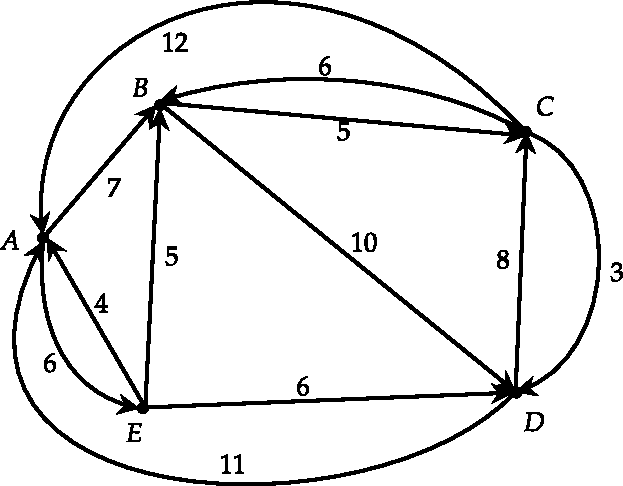
\includegraphics[scale=0.6]{Images/Dijkstra.pdf}
\end{center}
The weighted adjacency matrix of the graph is
\begin{equation*}
W = \kbordermatrix{
	&	A & B & C & D & E\\
	A & 0 & 7 & \infty & \infty & 6\\
	B & \infty & 0 & 5 & 10 & \infty\\
	C & 12 & 6 & 0 & 3 & \infty\\
	D & 11 & \infty & 8 & 0 & \infty\\
	E & 4 & 5 & \infty & 6 & 0
}.
\end{equation*}

The results of applying the algorithm are tabulated below and the tree of shortest paths is also shown.

\begin{center}
\begin{tabular}{cc}

	\begin{minipage}{5cm}
	$\begin{array}{r|cccc}
	 	 &		A	&	C	&	D	&	E\\
	\hline
	B(0) &	\infty_B	&	\boxed{5_B}	&	10_B	&	\infty_B\\
	C(5) &	17_C	&	\_	&	\boxed{8_C}	&	\infty_B\\
	D(8) &	\boxed{17_C}	&	\_	&	\_	&	\infty_B\\
	A(17)&	\_	&	\_	&	\_	&	23_A\\
	\hline
	B	&	17_C	&	5_B	&	8_C	&	23_A
	\end{array}$
	\end{minipage}
&
	\begin{minipage}{5cm}
		\centering
	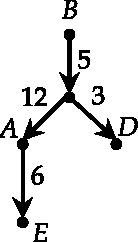
\includegraphics[scale=0.7]{Images/ShortestPaths.pdf}
	\end{minipage}

\end{tabular}
\end{center}

\end{Example}


%\begin{appendices}
%
%\end{appendices}